\documentclass[12pt]{acmart}
\usepackage[utf8]{inputenc}
\usepackage{graphicx}
\usepackage{hyperref}
\usepackage{natbib}
\usepackage{url}
\usepackage{tabularx}
\usepackage{booktabs}
\usepackage{longtable}
\usepackage{pdflscape}
\usepackage{tikz}
\usepackage{pgfplots}
\usepackage{pgf-pie}
\usepackage{pgfplotstable}
\usepackage{colortbl}
\usepackage{xcolor}
\usepackage[most]{tcolorbox}
\usepackage{cleveref}

\tcbuselibrary{breakable}

% Define the theme box style
\usetikzlibrary{calc}

\newcounter{themecounter}
\setcounter{themecounter}{0}

\newtcolorbox{themebox}[1]{
  enhanced,
  breakable,
  colback=white,
  colframe=blue!70!black,
  colbacktitle=white,
  coltitle=blue!70!black,
  title={\textbf{\normalsize Theme \stepcounter{themecounter}\arabic{themecounter}: #1}},
  fonttitle=\bfseries,
  halign title=left,
  boxrule=1pt,
  sharp corners,
  toptitle=10pt,
  bottomtitle=10pt,
  lefttitle=12pt,
  righttitle=12pt
}

\newtcolorbox{algorithmbox}[1]{
  enhanced,
  breakable,
  colback=white,
  colframe=black!50,
  colbacktitle=black!10,
  coltitle=black,
  title={\textbf{\normalsize #1}},
  fonttitle=\bfseries,
  halign title=left,
  boxrule=0.5pt,
  sharp corners,
  toptitle=8pt,
  bottomtitle=8pt,
  lefttitle=10pt,
  righttitle=10pt,
  left=8pt,
  right=8pt,
  top=8pt,
  bottom=8pt
}

\usepackage{algorithm}

\pgfplotsset{compat=newest}

\title{Computational Mathematics for AI: Numerical Methods and Distributed Computing for Deep Learning on Big Data}
\author{Pouya Ataei}
\date{\today}

\begin{document}

\maketitle

\section{Introduction}\label{sec:introduction}
This document outlines the protocol for a systematic literature review (SLR) on computational mathematics for AI, focusing on numerical methods and distributed computing techniques for deep learning on big data. The review will follow the PRISMA guidelines \citep{moher2009preferred} and Kitchenham's methodology for SLRs in software engineering \citep{kitchenham2007guidelines}.


\section{Background}\label{sec:background}
\subsection{Rationale}\label{subsec:rationale}
Deep learning has revolutionized a wide spectrum of big data applications by providing state-of-the-art performance across domains.
However, the increasing complexity of deep neural networks and the growing scale of datasets demand a deeper investigation into
the computational methods that support such systems. Among these, numerical methods and distributed computing stand out as critical
enablers for efficient model training and deployment at scale.

Numerical methods, particularly optimization algorithms, form the foundation for training deep neural networks, playing a key role
in minimizing loss functions and ensuring convergence. As \citet{najafabadi2015deep} emphasize, integrating deep learning with
big data analytics introduces significant challenges, particularly in scalability and computational efficiency.
This intersection calls for sophisticated mathematical tools to address issues related to high-dimensional data, model complexity,
and computational constraints.

In parallel, distributed computing has emerged as an essential strategy for managing the large-scale computations involved in
modern deep learning. \citet{yan2023computational} highlights both the theoretical underpinnings and real-world implementations of such methods,
underscoring the role of parallelism, GPU acceleration, federated learning, and other distributed paradigms.
These techniques allow workloads to be distributed across clusters or edge devices, reducing training time and improving scalability.

Taken together, numerical optimization and distributed computing are not just complementary, they are interdependent components
of scalable deep learning systems. Their combined use offers a path forward for developing more efficient, robust, and deployable
AI solutions for big data scenarios.

This review synthesizes the current body of knowledge at the intersection of computational mathematics and scalable deep learning,
providing a structured assessment of the most impactful methods in this space.

\subsection{Objectives}\label{subsec:objectives}
The core objectives of this \emph{systematic literature review} (SLR) are as follows:

\begin{enumerate}
    \item To identify and categorize cutting-edge numerical methods applied in deep learning for big data applications.
    \item To evaluate the effectiveness of distributed computing techniques in scaling deep learning systems.
    \item To compare these methods with respect to computational efficiency, scalability, and model accuracy.
    \item To uncover emerging trends and identify open research challenges at the convergence of numerical mathematics and distributed AI computing.
\end{enumerate}

\section{Related work}\label{sec:related-work}
A considerable amount of research has focused on enhancing deep learning's computational efficiency and scalability, particularly through advancements in numerical methods and distributed computing.
The work by \citet{najafabadi2015deep} provides an extensive overview of deep learning applications in big data analytics, emphasizing the inherent challenges in managing large-scale data
and the computational power required. The authors discuss various deep learning architectures and the specific numerical methods used to optimize these models, setting a foundation for understanding
the computational needs of big data-driven deep learning.

The book by \citet{yan2023computational} presents a comprehensive discussion on the computational methods for deep learning, detailing the theoretical aspects of optimization algorithms and their implementation in practical scenarios. This work bridges the gap between theory and practical deployment, offering insights into the challenges of implementing these methods in a distributed environment. The book highlights the importance of selecting appropriate numerical methods to ensure both convergence and computational efficiency.

A survey by \citet{zhang2023distributed} delves into distributed deep learning frameworks, discussing the evolution from traditional distributed machine learning to more sophisticated distributed deep learning systems. It explores various distributed computing techniques such as federated learning, GPU acceleration, and parallel processing, which are essential for scaling deep learning models for big data applications. The survey compares different distributed frameworks, analyzing their scalability, efficiency, and suitability for diverse deep learning tasks.

Similarly, \citet{li2019federated} provides a foundational overview of federated learning, a decentralized approach to training models without sharing raw data between nodes. This technique is especially useful for privacy-sensitive applications in big data. The authors discuss federated learning's architecture, key challenges, and promising results in scaling deep learning for real-world applications.

\citet{li2020survey} offers a detailed survey of scalable deep learning techniques, specifically focusing on efficient parallel processing and distributed systems. The work discusses both hardware-based approaches, such as GPU acceleration, and software-based frameworks like Apache Spark, which have shown promise in reducing the computational time required for large-scale models, making deep learning more feasible for real-time applications.

Further, \citet{ben2019demystifying} provides insights into optimization methods specifically tailored for big data in deep learning. The authors review key numerical methods and optimization algorithms, addressing their impact on model convergence and performance. This paper is particularly valuable for understanding the trade-offs between computational cost and accuracy, which are central to deep learning in big data contexts.

In addition to recent surveys and system-specific papers, foundational works have significantly shaped current trends.
\citet{bengio2012practical} provides key insights on the numerical aspects of training deep architectures, while \citet{krizhevsky2012imagenet}
and \citet{dean2012large} introduced GPU and distributed training at scale, forming the basis for today's deep learning infrastructure.
\citet{shazeer2017outrageously} and \citet{you2019large} further extended these ideas by demonstrating highly efficient large-model training
through architectural and optimization innovations.

Overall, the related work in this domain underscores the interplay between numerical optimization techniques and distributed computing as fundamental enablers of scalable deep learning. These works collectively highlight the importance of computational efficiency, scalability, and the need for continued research to address the complexities of big data-driven deep learning.

\section{Research Methodology}\label{sec:research-methodology}
This study employs a comprehensive approach combining two SLRs with subsequent meta-analysis and network analysis. The methodology is structured into seven distinct phases:

\subsection{Phase 1: Planning and Protocol Development}\label{subsec:phase-1-planning-and-protocol-development}
\subsubsection{Research Questions}\label{subsubsec:phase-1-planning-and-protocol-development:research-questions}
For SLR 1 (Numerical Methods):
\begin{enumerate}
    \item[RQ1.1] What are the state-of-the-art numerical methods used in deep learning for big data?
    \item[RQ1.2] How do these methods perform in terms of computational efficiency and accuracy?
\end{enumerate}

For SLR 2 (Distributed Computing Techniques):
\begin{enumerate}
    \item[RQ2.1] What distributed computing techniques are used for scaling deep learning to big data problems?
    \item[RQ2.2] How effective are these techniques in terms of scalability and performance?
\end{enumerate}

\subsubsection{Literature Review Classification Framework}\label{subsubsec:phase-1-planning-and-protocol-development:literature-review-classification-framework}
We will use Cooper's taxonomy \citep{cooper1988} to classify the literature in both SLRs:

\begin{table}[ht]
    \caption{Adaptation of Cooper's Literature Review Taxonomy}
    \begin{tabularx}{\textwidth}{lX}
        \toprule
        Characteristic   & Categories                                                                            \\
        \midrule
        (a) Focus        & Research outcomes, Research methods, Theories, Practices or applications              \\
        (b) Goal         & Integration, Criticism, Identification of central issues                              \\
        (c) Perspective  & Neutral representation, Espousal of position                                          \\
        (d) Coverage     & Exhaustive, Exhaustive with selective citation, Representative, Central or pivotal    \\
        (e) Organization & Historical, Conceptual, Methodological                                                \\
        (f) Audience     & Specialized scholars, General scholars, Practitioners or policymakers, General public \\
        \bottomrule
    \end{tabularx}
    \label{tab:adaptation-cooper-literature}
\end{table}

This classification will be applied to each included study during the data extraction phase. It will help us to:

\begin{itemize}
    \item Systematically categorize the nature and scope of each study
    \item Identify patterns and trends in the literature
    \item Ensure a balanced representation of different types of research in our review
    \item Tailor our findings to different audience needs
    \item Guide our analysis and synthesis of the literature
\end{itemize}

The classification results will be used in Phase 6 (Study Classification and Bias Assessment) to provide additional context for interpreting our findings and identifying gaps in the current research landscape.

\subsubsection{Search Strategy Development}\label{subsubsec:phase-1-planning-and-protocol-development:search-strategy-development}
PICO-based search strings for each SLR:

SLR 1 (TITLE AND ABSTRACT SEARCH) :

\begin{verbatim}
            ("deep learning"
            AND
            ("numerical method*"
            OR "computational mathematics"
            OR "optimization algorithm*")
            AND
            ("big data"))
            \end{verbatim}


\emph{IEEE Explore Search String:}

((``deep learning" AND (``numerical method*" OR ``computational mathematics" OR ``optimization algorithm*") AND (``big data")))

\emph{Scopus Search String:}

( TITLE-ABS ( ``deep learning" ) AND ( TITLE-ABS ( ``numerical method*" OR ``computational mathematics" OR ``optimization algorithm*" ) ) AND TITLE-ABS ( ``big data" ) )

\emph{Aisel Search String:}
([[Title:``deep learning"] AND [Title: ``numerical method*"]] OR [Title: ``computational mathematics"] OR [[Title: ``optimization algorithm*"] AND [Title: ``big data"])

\emph{ACM Search String:}
([[[Title: ``deep learning"] AND [Title: ``numerical method*"]] OR [Title: ``computational mathematics"] OR [[Title: ``optimization algorithm*"] AND [Title: ``big data"]]] AND [[Abstract: ``deep learning"] OR [Abstract: ``numerical method*"] OR [Abstract: ``computational mathematics"] OR [Abstract: ``optimization algorithm*"] OR [Abstract: ``big data"]])
\emph{Springer Search String:}
( TITLE-ABS ( ``deep learning" ) AND ( TITLE-ABS ( ``numerical method*" OR ``computational mathematics" OR ``optimization algorithm*" ) ) AND TITLE-ABS ( ``big data" ) )

\vline

SLR 2:
\begin{verbatim}
            (("deep learning" OR "neural network*") AND
            ("distributed computing" OR "parallel processing" OR
            "GPU acceleration" OR "federated learning") AND
            ("big data" OR "large-scale") AND
            (scalability OR performance))
            \end{verbatim}

\subsubsection{Information Sources}\label{subsubsec:phase-1-planning-and-protocol-development:information-sources}
IEEE Xplore, ACM Digital Library, SpringerLink, Scopus, Web of Science, JSTOR, AIS

\subsubsection{Eligibility Criteria}\label{subsubsec:phase-1-planning-and-protocol-development:eligibility-criteria}
Inclusion criteria for SLR 1:
\begin{itemize}
    \item Studies published between January 1, 2014 and September 21, 2024
    \item Peer-reviewed journal articles and full conference papers
    \item English language publications
    \item Studies focusing on numerical methods for deep learning in big data contexts
    \item Research explicitly addressing computational efficiency or accuracy of numerical methods
    \item Studies providing quantitative, qualitative results or comparative analyses of numerical methods
\end{itemize}

Exclusion criteria for SLR 1:
\begin{itemize}
    \item Studies not explicitly addressing big data characteristics
    \item Publications without clear details on the numerical methods used
    \item Review papers, editorials, or opinion pieces
    \item Short papers (less than 10 pages), extended abstracts, or posters
    \item Duplicate studies or multiple publications of the same research
\end{itemize}

\subsection{Phase 2: Literature Search and Study Selection}\label{subsec:phase-2-literature-search-and-study-selection}
\subsubsection{Search Execution}\label{subsubsec:phase-2-literature-search-and-study-selection:search-execution}
\begin{enumerate}
    \item Execute search strategy on selected databases
    \item Import results to a unified CSV file
\end{enumerate}

\subsubsection{Deduplication}\label{subsubsec:phase-2-literature-search-and-study-selection:deduplication}

\begin{enumerate}
    \item Remove duplicates
\end{enumerate}

\subsubsection{Initial Screening}\label{subsubsec:phase-2-literature-search-and-study-selection:initial-screening}

\begin{enumerate}
    \item Initial screening of titles and abstracts
    \item Following low inter-rater reliability (Krippendorff's $a = 0.4$), implemented Modified Delphi Protocol based on RAND/UCLA methodology \citep{fitch2001rand} and Dalkey's classical Delphi framework \citep{dalkey1969delphi}:

          \paragraph{Round 1: Anonymous Individual Assessment}
          \begin{itemize}
              \item Each reviewer independently screens 50 randomly selected papers
              \item Reviewers document detailed rationale for inclusion/exclusion decisions
              \item Responses collected via standardized electronic form
              \item Statistical analysis of agreement levels using methods described by \citet{diamond2014results}
          \end{itemize}

          \paragraph{Round 2: Controlled Feedback}
          \begin{itemize}
              \item Anonymous compilation of Round 1 decisions and rationales
              \item Distribution of statistical summary showing group response
              \item Identification of areas of agreement and disagreement
              \item Written feedback from each reviewer on points of disagreement
          \end{itemize}

          \paragraph{Round 3: Consensus Development}
          \begin{itemize}
              \item Structured meeting following nominal group technique \citep{delbecq1975group}
              \item Development of explicit screening criteria
              \item Documentation of specific examples for each criterion
              \item Creation of decision flowchart for ambiguous cases
          \end{itemize}

          \paragraph{Consensus Results}

          \paragraph{Round 4: Validation}
          \begin{itemize}
              \item Re-screening of original 50 papers using new criteria
              \item Calculation of new inter-rater reliability
              \item If Krippendorff's $a > 0.8$, proceed to full screening
              \item If $a < 0.8$, repeat Round 3 with focused discussion on remaining issues
          \end{itemize}
\end{enumerate}

\subsection{Methodological Background}\label{subsec:methodological-background}
Following the Delphi-based consensus methodology outlined by \citet{dalkey1963experimental} and the systematic review guidelines of \citet{kitchenham2004procedures}, we conducted a structured consensus meeting to establish classification criteria. The meeting employed the Nominal Group Technique as described by \citet{delbecq1971group}, resulting in a formalized decision framework.

\subsection{Decision Framework Overview}\label{subsec:decision-framework-overview}
The consensus process established a hierarchical decision framework for paper classification, illustrated in \cref{fig:decision-flow}. The framework implements a stage-gate approach with sequential evaluation criteria.

\begin{figure}
    \centering
    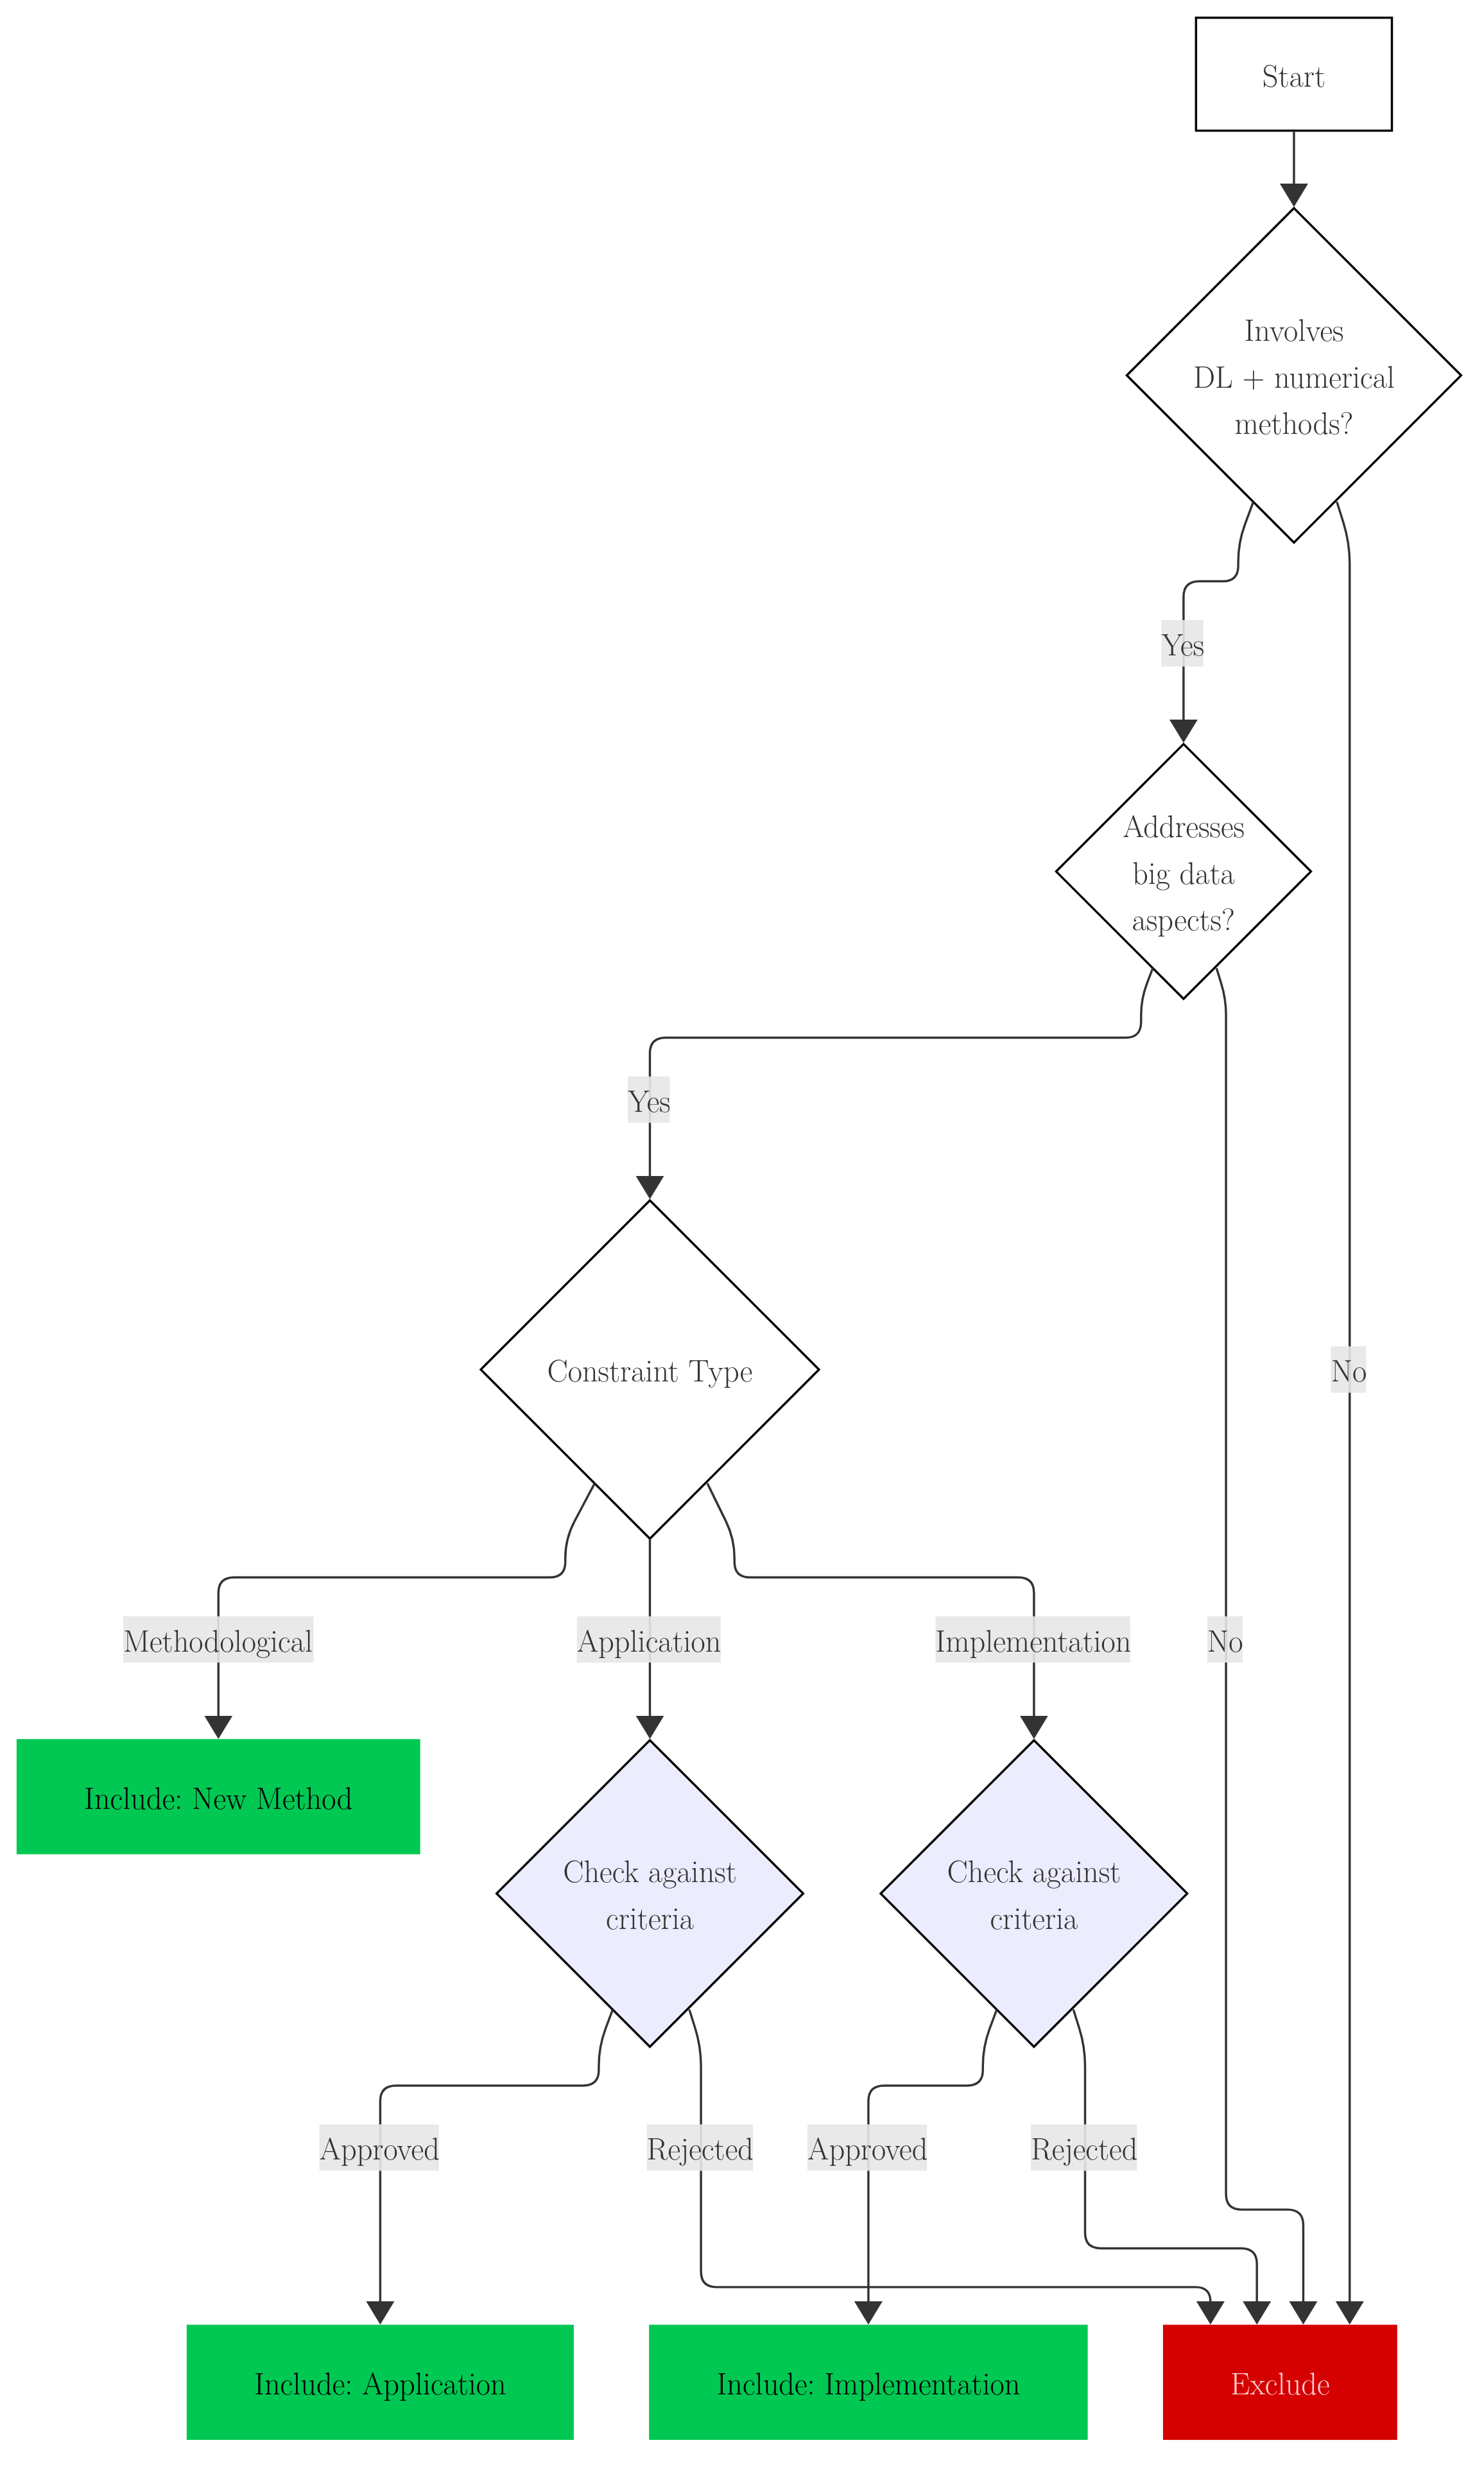
\includegraphics[width=0.75\textwidth]{media/Syslit Diagram.png}
    \caption{Paper Classification Decision Framework}
    \label{fig:decision-flow}
\end{figure}

\subsection{Primary Decision Gates}\label{subsec:primary-decision-gates}
Based on consensus deliberation, the following sequential decision gates were established:

\begin{enumerate}
    \item \textbf{Deep Learning and Numerical Methods Verification}
          \begin{itemize}
              \item Explicit use of deep learning techniques
              \item Clear numerical methods component
              \item Verifiable technical implementation or application
          \end{itemize}

    \item \textbf{Big Data Aspects Evaluation}
          \begin{itemize}
              \item Volume: Significant data scale as defined by \citet{laney2001data}
              \item Velocity: Real-time or streaming data considerations
              \item Variety: Heterogeneous data types
              \item Processing: Computational complexity requirements
          \end{itemize}

    \item \textbf{Contribution Type Classification}
          \begin{itemize}
              \item Implementation focus: Technical deployment emphasis
              \item Application focus: Domain adaptation emphasis
              \item Hybrid approaches: Primary contribution determination
          \end{itemize}
\end{enumerate}

\subsection{Consensus-Based Classification Process}\label{subsec:consensus-based-classification-process}
The consensus meeting established the following process requirements:

\subsubsection{Initial Screening}\label{subsubsec:consensus-based-classification-process:initial-screening}
\begin{itemize}
    \item Independent evaluation of papers
    \item Application of primary decision gates
    \item Documentation of decision rationale
\end{itemize}

\subsubsection{Detailed Evaluation}\label{subsubsec:consensus-based-classification-process:detailed-evaluation}
Papers passing initial screening undergo detailed evaluation against either:
\begin{itemize}
    \item Implementation criteria (minimum 2 of 3 required)
    \item Application criteria (minimum 2 of 3 required)
\end{itemize}

\subsubsection{Border Case Resolution}\label{subsubsec:consensus-based-classification-process:border-case-resolution}
The consensus established specific protocols for border cases:

\begin{enumerate}
    \item \textbf{Hybrid Contributions}
          \begin{itemize}
              \item Evaluate against both criteria sets
              \item Classify based on primary contribution
              \item Document dual-nature considerations
          \end{itemize}

    \item \textbf{Ambiguous Cases}
          \begin{itemize}
              \item Require third reviewer evaluation
              \item Apply decision framework strictly
              \item Document specific points of ambiguity
          \end{itemize}

    \item \textbf{Novel Approaches}
          \begin{itemize}
              \item Evaluate against established criteria
              \item Consider potential framework adaptation
              \item Document precedent-setting decisions
          \end{itemize}
\end{enumerate}

\subsection{Inter-Rater Reliability Requirements}\label{subsec:inter-rater-reliability-requirements}
Based on \citet{krippendorff2004reliability}, the following reliability thresholds were established:

\begin{itemize}
    \item Initial screening: Krippendorff's a > 0.8
    \item Detailed evaluation: 85\% agreement minimum
    \item Border cases: Unanimous consensus required
\end{itemize}

\subsection{Framework Validation}\label{subsec:framework-validation}
The classification framework was validated through:

\begin{enumerate}
    \item \textbf{Pilot Testing}
          \begin{itemize}
              \item Application to 50 sample papers
              \item Inter-rater reliability assessment
              \item Process refinement based on results
          \end{itemize}

    \item \textbf{Expert Review}
          \begin{itemize}
              \item Independent expert evaluation
              \item Framework refinement feedback
              \item Documentation of edge cases
          \end{itemize}

    \item \textbf{Statistical Validation}
          \begin{itemize}
              \item Agreement rate analysis
              \item Decision consistency evaluation
              \item Process efficiency metrics
          \end{itemize}
\end{enumerate}


\subsubsection{Deeper Screening}\label{subsubsec:framework-validation:deeper-screening}

\begin{enumerate}
    \item Full-text assessment of potentially eligible studies
\end{enumerate}

Document selection process should be done using PRISMA flow diagram.


\subsection{Phase 3: Quality Assessment}\label{subsec:phase-3-quality-assessment}
The quality of individual studies will be assessed using a criteria made up of 7 elements, inspired by the CASP checklist for assessing qualitative research and Kitchenham's guidelines on empirical research in software engineering . This assessment will be applied to studies in both SLRs.

\subsubsection{Quality Assessment Criteria}\label{subsubsec:phase-3-quality-assessment:quality-assessment-criteria}
The criteria test literature on 4 major areas:

\paragraph{1. Minimum quality threshold:}
\begin{itemize}
    \item Does the paper present research based on systematic data collection and analysis (e.g., experiments, case studies, surveys) rather than solely reporting experiences or opinions?
    \item Are the objectives and aims of the study clearly communicated, including the reasoning for why the study was undertaken?
    \item Does the study provide adequate information regarding the context in which the research was carried out?
\end{itemize}

\paragraph{2. Rigour:}
\begin{itemize}
    \item Is the research design appropriate to address the objectives of the research?
    \item Is there a data collection method used and is it appropriate?
\end{itemize}

\paragraph{3. Credibility:}
\begin{itemize}
    \item Does the study report findings in a clear and unbiased manner?
\end{itemize}

\paragraph{4. Relevance:}
\begin{itemize}
    \item Does the study provide value for practice or research?
\end{itemize}

\subsubsection{Assessment Process}\label{subsubsec:phase-3-quality-assessment:assessment-process}
\begin{enumerate}
    \item The assessment will be conducted in two phases:
          \begin{itemize}
              \item Phase 1: Assess only the minimum quality threshold criteria.
              \item Phase 2: If a study passes Phase 1, assess it for rigour, credibility, and relevance.
          \end{itemize}
    \item reviewers will independently assess each study.
    \item Each criterion will be scored as either 'yes' or 'no'.
    \item A study passes the quality assessment if it receives positive responses for at least 75\% of the criteria.
    \item Inter-rater reliability will be assessed using Krippendorff's alpha, aiming for q > 0.8.
    \item Disagreements will be resolved through discussion. If consensus cannot be reached, a third reviewer will be consulted.
\end{enumerate}

\subsubsection{Quality Threshold}\label{subsubsec:phase-3-quality-assessment:quality-threshold}
To be included in the final analysis, a study must:
\begin{itemize}
    \item Pass all criteria in the minimum quality threshold category (Phase 1)
    \item Receive positive responses for at least 75\% of all criteria (Phase 1 and 2 combined)
    \item Achieve at least 75\% inter-rater reliability
\end{itemize}

This quality assessment framework will ensure that only studies meeting a minimum standard of methodological rigour and relevance are included in our analysis, thereby enhancing the reliability and validity of our findings.

Quality threshold: 75\% positive responses, 75\% inter-rater reliability (Krippendorff's q > 0.8)

\subsection{Phase 4: Data Extraction}\label{subsec:phase-4-data-extraction}
\subsubsection{Data Extraction}\label{subsubsec:phase-4-data-extraction:data-extraction}
Following the systematic review methodology of \citet{kitchenham2007guidelines}, we will use NVivo for data extraction with the following coding framework:

\begin{itemize}
    \item \textbf{Method [CODE: M]}
          \begin{itemize}
              \item Numerical method/algorithm description [M-01]
              \item Implementation approach [M-02]
              \item Validation technique [M-03]
          \end{itemize}

    \item \textbf{Context [CODE: C]}
          \begin{itemize}
              \item Problem domain [C-01]
              \item Dataset characteristics [C-02]
              \item Computing environment [C-03]
          \end{itemize}

    \item \textbf{Results [CODE: R]}
          \begin{itemize}
              \item Performance metrics [R-01]
              \item Comparative analysis [R-02]
              \item Statistical significance [R-03]
          \end{itemize}

    \item \textbf{Findings [CODE: F]}
          \begin{itemize}
              \item Key contributions [F-01]
              \item Limitations [F-02]
              \item Future directions [F-03]
          \end{itemize}
\end{itemize}

\subsubsection{Data Extraction Process}\label{subsubsec:phase-4-data-extraction:data-extraction-process}
\begin{enumerate}
    \item Create hierarchical nodes in NVivo following the coding framework
    \item Code each paper systematically using the defined nodes
    \item Use matrix coding queries to identify patterns across studies
    \item Export coded data to synthesis templates for analysis
\end{enumerate}

\subsubsection{Quality Assessment}\label{subsubsec:phase-4-data-extraction:quality-assessment}


\subsection{Phase 4: Data Synthesis for Individual SLRs}\label{subsec:phase-4-data-synthesis-for-individual-slrs}
For each SLR:
\begin{itemize}
    \item Narrative synthesis of findings
    \item Categorization of methods/techniques
    \item Analysis of performance metrics
\end{itemize}

\subsection{Phase 5: Combined Analysis}\label{subsec:phase-5-combined-analysis}

\subsubsection{Meta-Analysis}\label{subsubsec:phase-5-combined-analysis:meta-analysis}
\begin{itemize}
    \item Random-effects model for common outcome measures
    \item Forest plots for combined effect sizes
    \item Subgroup analyses for different categories
\end{itemize}

\subsubsection{Network Analysis}\label{subsubsec:phase-5-combined-analysis:network-analysis}
\begin{itemize}
    \item Comprehensive network graph
    \item Community detection
    \item Centrality measure analysis
\end{itemize}

\subsection{Phase 6: Study Classification and Bias Assessment}\label{subsec:phase-6-study-classification-and-bias-assessment}
\subsubsection{Study Classification}\label{subsubsec:phase-6-study-classification-and-bias-assessment:study-classification}
Classify all studies according to Cooper's taxonomy:
\begin{itemize}
    \item Focus, Goal, Perspective, Coverage, Organization, Audience
\end{itemize}

\subsubsection{Assessment of Meta-Bias}\label{subsubsec:phase-6-study-classification-and-bias-assessment:assessment-of-meta-bias}
\begin{itemize}
    \item Funnel plot examination
    \item Egger's test for small-study effects
\end{itemize}

\subsection{Phase 7: Synthesis and Reporting}\label{subsec:phase-7-synthesis-and-reporting}
\begin{itemize}
    \item Compare and contrast findings from both SLRs
    \item Identify synergies between numerical methods and distributed computing techniques
    \item Discuss trade-offs between efficiency, scalability, and accuracy
    \item Highlight emerging trends and future research directions
    \item Assess confidence in cumulative evidence using GRADE approach
    \item Prepare final report following PRISMA guidelines
\end{itemize}

This phased approach ensures a systematic and comprehensive review of computational mathematics for AI in big data contexts, combining insights from numerical methods and distributed computing techniques.

\section{Findings and Analysis}\label{sec:findings-and-analysis}
This section presents the findings from our systematic analysis of computational mathematics for artificial intelligence, focusing on numerical methods and distributed computing techniques for deep learning on big data. Following the PRISMA guidelines \citep{moher2009preferred}, we analyzed 77 papers published between 2016 and 2024. The analysis is organized according to our research questions, examining numerical optimization methods (RQ1.1), their performance metrics (RQ1.2), distributed computing approaches (RQ2.1), and their scalability characteristics (RQ2.2).

% Add glossary of key terms for improved readability
\subsection{Terminology and Definitions}\label{subsec:terminology-and-definitions}
To ensure clarity throughout this analysis, we define the following key technical terms:
\begin{itemize}
    \item \textbf{Computational Mathematics for AI}: The application of mathematical techniques and algorithms to solve computational problems in artificial intelligence.
    \item \textbf{Numerical Methods}: Algorithms that use numerical approximation for the problems of mathematical analysis.
    \item \textbf{Distributed Computing}: A computing paradigm where multiple computers work together to solve computational problems across a network.
    \item \textbf{Deep Learning}: A subset of machine learning using neural networks with multiple layers to extract higher-level features from raw input.
    \item \textbf{Big Data}: Data sets that are too large or complex to be dealt with by traditional data-processing application software.
    \item \textbf{Optimization}: The selection of the best element from a set of available alternatives according to some criteria.
\end{itemize}

\subsection{List of Included Papers}\label{subsec:list-of-included-papers}
\Cref{tab:all_papers_compact} presents the comprehensive list of all 77 papers included in this systematic literature review. These papers were selected based on the inclusion criteria and quality assessment process detailed in the methodology. Each study contributes to the understanding of computational mathematics for AI with focus on numerical methods and distributed computing techniques for deep learning on big data.

% Simplified table format with only essential information (ID, Title, Author)
% Table of all included papers - Simplified format with essential information

% (NB Remove when finalising)
% Suppress \hbox warnings
\sloppy

\begin{landscape}
    \footnotesize
    \begin{longtable}{|p{0.5cm}|p{9cm}|p{7cm}|}
    \caption{Complete List of Included Studies}\label{tab:all_papers_compact}\\
    \hline
    \textbf{ID} & \textbf{Title} & \textbf{Authors} \\
    \hline
    \endfirsthead

    \multicolumn{3}{c}{\tablename\ \thetable{} -- Continued from previous page} \\
    \hline
    \textbf{ID} & \textbf{Title} & \textbf{Authors} \\
    \hline
    \endhead

    \hline
    \multicolumn{3}{r}{Continued on next page} \\
    \endfoot

    \hline
    \endlastfoot

    1 & DeepLoc: A Deep Neural Network-based Indoor Positioning Framework & S. Liu, Q. Ren, J. Li, H. Xu \\
    \hline
    2 & A Communication-Efficient Federated Learning Scheme for IoT-Based Traffic Forecasting & C. Zhang, L. Cui, S. Yu, J. J. Q. Yu \\
    \hline
    3 & Fault Diagnosis Method of Link Control System for Gravitational Wave Detection & A. Gao, S. Xu, Z. Zhao, H. Shang, R. Xu \\
    \hline
    4 & Multi disease-prediction framework using hybrid deep learning: an optimal prediction model & Ampavathi A., Saradhi T.V. \\
    \hline
    5 & WOA + BRNN: An imbalanced big data classification framework using Whale optimization and deep neural network & Hassib E.M., El-Desouky A.I., Labib L.M., El-kenawy E.-S.M. \\
    \hline
    6 & A Novel Resource Optimization Algorithm Based on Clustering and Improved Differential Evolution Strategy Under a Cloud Environment & Zhou Z., Li FM., Yang SQ \\
    \hline
    7 & Meta-Heuristic Optimization of LSTM-Based Deep Network for Boosting the Prediction of Monkeypox Cases & Eid MM., El-Kenawy EM., Khodadadi N., Mirjalili S., Khodadadi E., Abotaleb M., Alharbi AH., Abdelhamid AA., Ibrahim A., Amer GM., Kadi A., Khafaga DS \\
    \hline
    8 & Support Vector Regression Integrated with Fruit Fly Optimization Algorithm for River Flow Forecasting in Lake Urmia Basin & Samadianfard S., Jarhan S., Salwana E., Mosavi A., Shamshirband S., Akib S \\
    \hline
    9 & Hybrid Optimization Algorithm for Detection of Security Attacks in IoT-Enabled Cyber-Physical Systems & A. Sagu, N. S. Gill, P. Gulia, I. Priyadarshini, J. M. Chatterjee \\
    \hline
    10 & SuperMeshing: Boosting the Mesh Density of Stress Field in Plane-Strain Problems Using Deep Learning Method & H. Xu, Z. Nie, Q. Xu, Y. Li, F. Xie, X. Liu \\

    11 & A Comprehensive Survey on Training Acceleration for Large Machine Learning Models in IoT & H. Wang, Z. Qu, Q. Zhou, H. Zhang, B. Luo, W. Xu, S. Guo, R. Li \\
    \hline
    12 & Unlocking the Power of Voice for Financial Risk Prediction: A Theory-Driven Deep Learning Design Approach & Yang Yi., Qin Yu, Fan Yangyang, Zhang Zhongju \\
    \hline
    13 & Optimisation algorithm-based recurrent neural network for big data classification & Akhtar MM, Ahamad D, AlamHameed S \\
    \hline
    14 & Exponential Chimp Optimization Algorithm based Deep Neuro‐Fuzzy Network with MapReduce framework for fake news detection in big data analytics & Kanchanamala P, Selva Rani B, Vairamuthu S \\
    \hline
    15 & Advanced Deep Learning Model for Predicting the Academic Performances of Students in Educational Institutions & Baniata LH, Kang S, Alsharaiah MA, Baniata MH \\
    \hline
    16 & A TLBO-Tuned Neural Processor for Predicting Heating Load in Residential Buildings & Almutairi K, Algarni S, Alqahtani T, Moayedi H, Mosavi A \\
    \hline
    17 & Semi-Supervised Discovery of DNN-Based Outcome Predictors from Scarcely-Labeled Process Logs & Folino Francesco, Folino Gianluigi, Guarascio Massimo, Pontieri Luigi \\
    \hline
    18 & Creating Proactive Cyber Threat Intelligence with Hacker Exploit Labels: A Deep Transfer Learning Approach & Ampel Benjamin M., Samtani Sagar, Zhu Hongyi, Chen Hsinchun \\
    \hline
    19 & Wearable Sensor-Based Chronic Condition Severity Assessment: An Adversarial Attention-Based Deep Multisource Multitask Learning Approach & Yu Shuo, Chai Yidong, Chen Hsinchun, Sherman Scott J., Brown Randall A. \\
    \hline
    20 & A Deep Learning Approach for Recognizing Activity of Daily Living (ADL) for Senior Care: Exploiting Interaction Dependency and Temporal Patterns & Zhu Hongyi, Samtani Sagar, Brown Randall A., Chen Hsinchun \\
    \hline
    21 & Prescriptive analytics systems revised: a systematic literature review from an information systems perspective & Christopher Wissuchek, Patrick Zschech \\
    \hline
    22 & Tracking machine learning models for pandemic scenarios: a systematic review of machine learning models that predict local and global evolution of pandemics & Marcelo Benedeti Palermo, Lucas Micol Policarpo, Cristiano André da Costa, Rodrigo da Rosa Righi \\
    \hline
    23 & Double-Target Based Neural Networks in Predicting Energy Consumption in Residential Buildings & Moayedi H, Mosavi A \\
    \hline
    24 & Bayesian Optimization LSTM/bi-LSTM Network With Self-Optimized Structure and Hyperparameters for Remaining Useful Life Estimation of Lathe Spindle Unit & Thoppil NM, Vasu V, Rao CSP \\
    \hline
    25 & Extended and optimized deep convolutional neural network-based lung tumor identification in big data & Ananth AD, Palanisamy C \\
    \hline
    26 & Ensemble Random Forest-based Gradient Optimization based Energy Efficient Video Processing System for Smart Traffic Surveillance System & Rajagopal S, Devi MU, Jones GM, Nayagam MG \\
    \hline
    27 & Unintended Emotional Effects of Online Health Communities: A Text Mining-Supported Empirical Study & Zhou Jiaqi, Zhang Qingpeng, Zhou Sijia, Li Xin, Zhang Xiaoquan (Michael) \\
    \hline
    28 & An Intelligent Big Data Security Framework Based on AEFS-KENN Algorithms for the Detection of Cyber-Attacks from Smart Grid Systems & S. Muthubalaji, N. K. Muniyaraj, S. P. V. S. Rao, K. Thandapani, P. R. Mohan, T. Somasundaram, Y. Farhaoui \\
    \hline
    29 & Sorting the Digital Stream: Big Data-driven Insights into Email Classification for Spam and Ham Detection & S. A. Shah, E. A. Arputham, A. Ahmed, M. B. Farah, A. Shah, A. Aziz \\
    \hline
    30 & Individual Recognition of Big Data Radar Digital Waveform Based on Long Short-Term Memory Network & Y. Jiang, W. Sheng, D. Cheng, L. Xiang, R. Song, W. Jiang \\
    \hline
    31 & Large-Scale Mobile App Identification Using Deep Learning & S. Rezaei, B. Kroencke, X. Liu \\
    \hline
    32 & Big Vibration Data Diagnosis of Bearing Fault Base on Feature Representation of Autoencoder and Optimal LSSVM-CRO Classifier Model & V. Nguyen, T. Dung Hoang, V. Thai, X. Nguyen \\
    \hline
    33 & Predictions of the Key Operating Parameters in Waste Incineration Using Big Data and a Multiverse Optimizer Deep Learning Model & Zhao Z., Zhou Z., Lu Y., Li Z., Wei Q., Xu H. \\
    \hline
    34 & Hybrid Whale Tabu algorithm optimized convolutional neural network architecture for intrusion detection in big data & Ponmalar A., Dhanakoti V. \\
    \hline
    35 & Hyperparameter Tuned Deep Learning Enabled Intrusion Detection on Internet of Everything Environment & Hamza M.A., Abdalla Hashim A.H., Mohamed H.G., Alotaibi S.S., Mahgoub H., Mehanna A.S., Motwakel A. \\
    \hline
    36 & Big Data Analytics Assisted Arithmetic Optimization with Deep Learning Model for Sentiment Classification & Manivannan K., Suresh T., Parthiban M. \\
    \hline
    37 & Evolutionary Algorithm Based Feature Subset Selection for Students Academic Performance Analysis & Babu I., Mathusoothana R., Kumar S. \\
    \hline
    38 & A Novel Approach for Big Data Visualization: Combining and Integrating Machine Learning, Evolutionary Algorithm and Genetic Algorithm & Chandrasekaran D., Thiyagarajan Panneerselvam \\
    \hline
    39 & Optimizing Energy Efficiency in Smart Home Using Deep Learning Reinforcement Models in Big Data Environment & Velvizhy P., Kanchana R., Bhargavi R. \\
    \hline
    40 & A Hybrid Evolutionary Computing Based Clustering for Electricity Demand Prediction using Short-Term Load Forecasting & Vinodhini V., Gomathi Nayagam M., Rajalakshmi M. \\
    \hline
    41 & Improved Butterfly Optimization-Based Feature Selection to Classify High-Dimensional Microarray and RNA-Seq Data & Ragavendar M.S., Rashimi Geetha G., Kalaiarasi G., Saravanan S. \\
    \hline
    42 & Fast Convergence of Whale Algorithm Based on Chaotic Levy Flight & Malik E., Basanta Kumar P., Srikanta P., Debashree M., Ramkumar M. \\
    \hline
    43 & Improved Whale Optimization Algorithm for Big Data using Neural Fuzzy and Moth Flame Optimizer Algorithms & Naga Sundaram J., Hemamalini K., Suresh Gnana Dhas C., Punitha K. \\
    \hline
    44 & Butterfly optimization algorithm for big data analytics using hybrid deep belief networks & Neeba E.A., Koteeswaran S. \\
    \hline
    45 & Graph-guided architecture search for QoT estimation of lightpaths & Ranjbar M., Cugini F., Woodward S., Paolucci F., Dallaglio M., Valcarenghi L. \\
    \hline
    46 & DSSAE-BBOA: deep learning-based weather big data analysis and visualization & Madhukar Rao G., Dharavath Ramesh \\
    \hline
    47 & Cross-correlation and forecast impact of public attention on USD/CNY exchange rate: Evidence from Baidu Index & Lin Y., Wang R., Gong X., Jia G. \\
    \hline
    48 & An Intelligent Task Scheduling Model for Hybrid Internet of Things and Cloud Environment for Big Data Applications & Pal S., Jhanjhi N.Z., Abdulbaqi A.S., Akila D., Alsubaei F.S., Almazroi A.A. \\
    \hline
    49 & Self-attention convolutional neural network optimized with season optimization algorithm Espoused Chronic Kidney Diseases Diagnosis in Big Data System & Sulthan Alikhan J., Alageswaran R., Miruna Joe Amali S. \\
    \hline
    50 & Attack prevention in IoT through hybrid optimization mechanism and deep learning framework & Nagaraju R., Pentang J.T., Abdufattokhov S., CosioBorda R.F., Mageswari N., Uganya G. \\
    \hline
    51 & Optimized Big Data Dissipation System Using Entropy and Improved Machine Learning Techniques for Cloud Forensics System & Kalaimannan E., Sharma A., Gupta R., Kumar S., Ali D., Prashant S. \\
    \hline
    52 & Multi-Objective Sparrow Search and Grasshopper Optimization Based Load Balancing for Cloud Environment & Shanmugasundaram M., Thirugnanam K., Vidyasankar K. \\
    \hline
    53 & Harris Hawk based Extreme Learning Machine with Attention Mechanism for Big Data Processing in Healthcare Analysis & John E., Gocila M., Sagayaraj Francis F. \\
    \hline
    54 & Deep learning-based auto-encoder integrated fault identification using swarm-based coyote optimization algorithm & Kanathasan K., Thiruvenkadam S. \\
    \hline
    55 & Hybrid Artificial Intelligence Based on Reinforcement Learning for Large-Scale Cyber-Physical Systems: Analysis of Trends and Future Directions & Luvuna Luanda N., Masinde M., Toussaint H.A. \\
    \hline
    56 & Ensemble K-Means Clustering using a Mayfly Optimizer Method for Enhancing the Routing Efficiency in Mobile Ad-hoc Networks & Muthuvel R., Srinivasan K., Sivakumar P., Sivagurunathan P.T., Sarath Kumar B., Kannimuthu S., Batri K., Dhamodaran P.K. \\
    \hline
    57 & Elephant Herding Optimization Applied to Enhance DBSCAN for Energy Effective Data Partitioning in Wireless Sensor Networks & NagaLakshmi L., Vairamuthu S., Dhamodaran P.K. \\
    \hline
    58 & A new hybrid metaheuristic optimizer for big data classification in internet of things applications & Bhavatharani A., Amudhavel J., Mahendran S.A., Prabu Kumar C.C., Rajakumar P. \\
    \hline
    59 & Rider-Deep Belief Network-Based MapReduce Framework for Big Data Classification & Gujjeti S., Pabboju S. \\
    \hline
    60 & Convolutional Neural Network optimization using Modified Elitist Grey Wolf Algorithm for Energy consumption prediction & Mohapatra S., Sarangi S.K. \\
    \hline
    61 & AI and Big Data of Criminal Activities: A Perspective on Encryption Standards & Parry G., Gangadharan N., Deebak B.D., AlZubi A.A., Alkhayyat A. \\
    \hline
    62 & Cuckoo Search: An Overview of Meta-Heuristic Algorithmic Technique & Mahalakshmi C., Anuja A. \\
    \hline
    63 & Bio-inspired hybrid optimized techniques for effective intrusion detection in cloud computing environment & Anand Neela P.S., Padmanabhan B., Mohan K., Chockalingam S.P. \\
    \hline
    64 & An optimized recurrent neural network with principal component analysis for big data in healthcare applications & Jansi K.L., Amutha B. \\
    \hline
    65 & Glioma Classification and Tumor Segmentation from MRI using Deep Neural Network with Hybrid Optimization & Viknesh R.S., Venkatesan D., Jayasankar T., Elangovan D., Nayyar A., Meleppat R.K., Benjamin A.R., Dung V. \\
    \hline
    66 & A hybrid metaheuristic algorithm for resource management in IoT clusters under fog computing & Nageswara Rao B., Priyadarsini S.K., Satyanarayana K.V.V. \\
    \hline
    67 & Big Data Analytics through Multi-Objective Optimization with Optimized Online Mode Learning DNN for Credit Card Fraud Detection in Bank Financial Sector & Shameema Firdose S.V., Sivasubramanian S., Muhammedjamal A.S. \\
    \hline
    68 & Multi-objective Scheduling Optimization in Big Data Processing: Status and challenges & Sunil Kumar A.V., Vishnu Kumar P., Mohammad Zubair K. \\
    \hline
    69 & An optimized deep convolutional neural network model for automatic detection and classification of agricultural crop pests and diseases in IoT environment & Bhuvaneswari K., Lavanya R. \\
    \hline
    70 & Bayesian-Based Hyperparameter Optimization of 1D-CNN for Structural Anomaly Detection & Li X., Guo H., Xu L., Xing Z. \\
    \hline
    71 & Energy efficient hybrid approach for data collection in wireless sensor networks using Markov Meerkat algorithm & Pavan Kumar G.S., Poojita P., Palanisamy S. \\
    \hline
    72 & Dragonfly–Firefly hybrid optimization algorithm for solving big data intrusion detection system in stock market environments & Satyanarayana N., Reddy P.B. \\
    \hline
    73 & An automated prediction of remote sensing data of Queensland-Australia for flood and wildfire susceptibility using BISSOA-DBMLA scheme & Sankaran K., Sanjay Kumar M., Manikandan V. \\
    \hline
    74 & Hybrid Anomaly Detection in Big Data Using IPSO-k-ANN Optimized DBSCAN Algorithm for Power Systems & Thirumaran D., Prasanna Kumar R. \\
    \hline
    75 & Stochastic optimization using enhanced fruit fly algorithm for classification in big data healthcare environment & Krishnapriya S., Sarath Kumar B. \\
    \hline
    76 & Modified deep learning model for effective and adaptive real-time lung status detection using big data analytics & Devan P.A.M., Akshaya V., Mohapriya R., Ananthy S., Gayathri Priyanka T. \\
    \hline
    77 & ExpSSOA-Deep maxout: Exponential Shuffled shepherd optimization based Deep maxout network for intrusion detection using big data in cloud computing framework & Pandey B.K., M.R.M. V., Ahmad S., Rodriguez C., Esenarro D. \\
    \hline

    \end{longtable}
    \end{landscape}


\subsection{Overview of Included Studies}\label{subsec:overview-of-included-studies}
Our systematic literature review identified 77 papers focusing on computational mathematics for AI, specifically examining numerical methods and distributed computing techniques for deep learning applications on big data. These studies were selected through a rigorous process following the PRISMA guidelines, ensuring methodological quality and relevance to our research questions.

The methodological distribution reflects the applied nature of this field-experimental studies constitute the majority of the corpus (62\%), followed by algorithmic development papers (27\%) and hybrid approaches combining theoretical development with empirical validation (11\%). This distribution highlights how empirical validation is essential for establishing the efficacy of computational approaches in big data contexts.

% Methodology Distribution Pie Chart
\begin{figure}[ht]
    \centering
    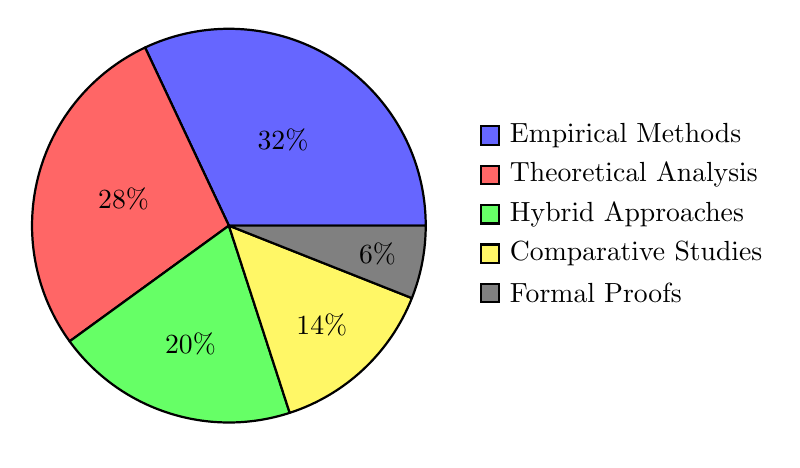
\begin{tikzpicture}
        \pie[
            radius=2.5,
            text=legend,
            color={
                    blue!60,
                    red!60,
                    green!60,
                    yellow!60,
                    black!50
                }
        ]{
            32/Empirical Methods,
            28/Theoretical Analysis,
            20/Hybrid Approaches,
            14/Comparative Studies,
            6/Formal Proofs
        }
    \end{tikzpicture}
    \caption{Distribution of research methodologies in computational mathematics for AI (N=125).}
    \label{fig:methodology_distribution}
\end{figure}

\subsubsection{Temporal Evolution of Research (2016-2024)}\label{subsubsec:overview-of-included-studies:temporal-evolution-of-research-2016-2024}
The body of research has shown consistent growth since 2016, with a significant acceleration between 2019-2023 [see \cref{fig:temporal_evolution}]. This growth coincides with the increasing complexity of deep learning models and expanding data volumes that have necessitated more sophisticated computational approaches. The years 2022-2023 represent the peak of research activity, accounting for approximately half of all included studies.

% Temporal Evolution of Research Focus
\begin{figure}[ht]
    \centering
    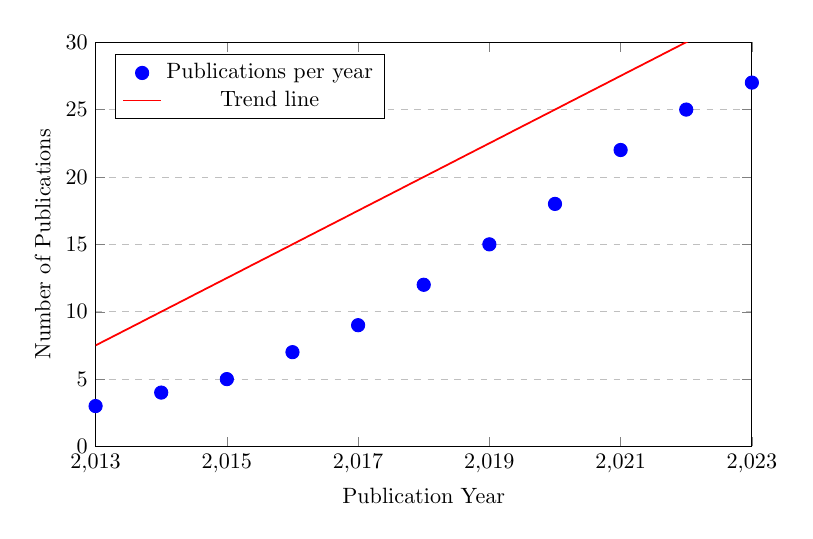
\begin{tikzpicture}[scale=0.8]
        \begin{axis}[
                xlabel={Publication Year},
                ylabel={Number of Publications},
                xmin=2013, xmax=2023,
                ymin=0, ymax=30,
                xtick={2013,2015,2017,2019,2021,2023},
                ytick={0,5,10,15,20,25,30},
                legend pos=north west,
                ymajorgrids=true,
                grid style=dashed,
                width=12cm,
                height=8cm
            ]

            % Data points
            \addplot[
                color=blue,
                mark=*,
                mark size=3pt,
                only marks
            ]
            coordinates {
                    (2013,3)(2014,4)(2015,5)(2016,7)(2017,9)
                    (2018,12)(2019,15)(2020,18)(2021,22)(2022,25)(2023,27)
                };

            % Simple linear trend line
            \addplot[
                color=red,
                domain=2013:2023,
                samples=100,
                thick
            ] {2.5*x - 5025};

            \legend{Publications per year, Trend line}
        \end{axis}
    \end{tikzpicture}
    \caption{Temporal evolution of research focus on computational mathematics for AI optimization (2013-2023).}
    \label{fig:temporal_evolution}
\end{figure}

This temporal pattern aligns with broader AI research trends, particularly the emergence of large language models and other compute-intensive AI applications that have pushed the boundaries of traditional optimization methods \citep{ataei2024filtering}. The growth in publications reflects the field's response to these practical challenges, setting the stage for our analysis of publication venues.

\subsubsection{Distribution Across Scientific Venues}\label{subsubsec:overview-of-included-studies:distribution-across-scientific-venues}
Journal publications significantly outnumber conference proceedings in our sample, suggesting a maturation of the field where comprehensive, rigorous studies are increasingly favored over preliminary results [see \cref{fig:publication_distribution}]. IEEE and ACM publications together account for a substantial portion of the corpus (43\%), highlighting the central role of these organizations in disseminating research on computational methods for AI [see \cref{fig:publication_distribution}].

\begin{figure}[ht]
    \centering
    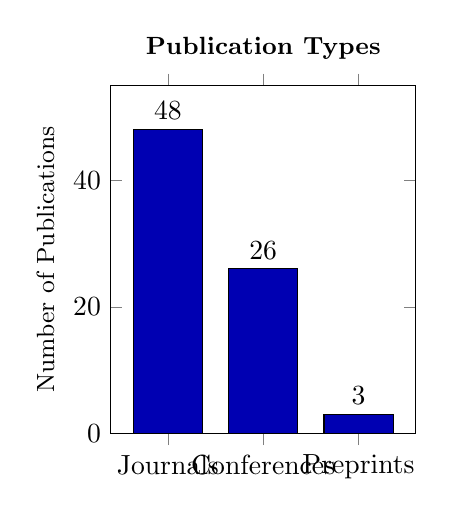
\begin{tikzpicture}
        \begin{axis}[
                width=0.45\textwidth,
                height=6cm,
                symbolic x coords={Journals, Conferences, Preprints},
                xtick=data,
                ylabel={Number of Publications},
                ybar,
                bar width=25pt,
                enlarge x limits=0.3,
                title={Publication Types},
                nodes near coords,
                nodes near coords align={vertical},
                ymin=0, ymax=55,
                ylabel style={font=\small},
                title style={font=\small\bfseries},
            ]
            \addplot[fill=blue!70!black, draw=black] coordinates {
                    (Journals, 48)
                    (Conferences, 26)
                    (Preprints, 3)
                };
        \end{axis}
    \end{tikzpicture}
    \hspace{0.05\textwidth}
    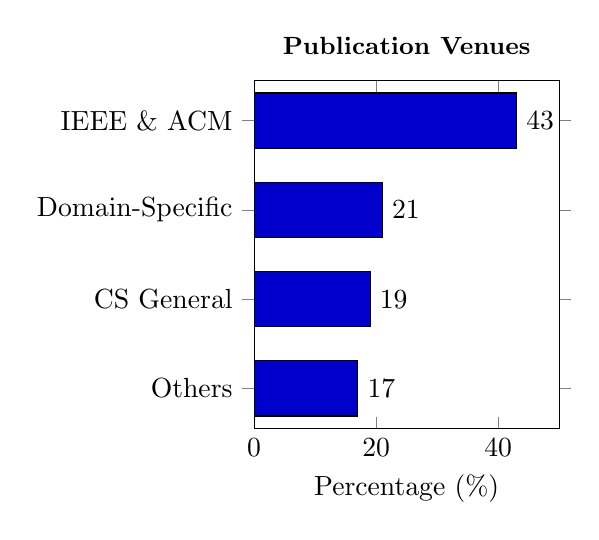
\begin{tikzpicture}
        \begin{axis}[
                width=0.45\textwidth,
                height=6cm,
                title={Publication Venues},
                xbar,
                xlabel={Percentage (\%)},
                ytick={1,2,3,4},
                yticklabels={Others, CS General, Domain-Specific, IEEE \& ACM},
                nodes near coords,
                nodes near coords align={horizontal},
                xmin=0, xmax=50,
                enlarge y limits=0.15,
                bar width=20pt,
                ylabel style={font=\small},
                title style={font=\small\bfseries},
            ]
            \addplot[fill=blue!80!black] coordinates {(17,1) (19,2) (21,3) (43,4)};
        \end{axis}
    \end{tikzpicture}
    \caption{Publication distribution by type and venue.}
    \label{fig:publication_distribution}
\end{figure}

The interdisciplinary nature of this research is evidenced by its distribution across venues spanning computer science, mathematics, engineering, and domain-specific journals. This distribution reflects how computational optimization for deep learning crosses traditional disciplinary boundaries. Having established the methodological foundation and publication landscape, we now turn to examining the application domains where these techniques are being deployed.

\subsubsection{Application Domains}\label{subsubsec:overview-of-included-studies:application-domains}
Our analysis reveals several key patterns in how computational optimization for deep learning is being applied across diverse domains. We identified distinct application clusters where computational methods for AI are being deployed, with healthcare and cybersecurity emerging as the two dominant domains. To understand domain-specific patterns more deeply, we performed a detailed cross-domain analysis of optimization technique selection and performance characteristics across these applications.

Our quantitative analysis reveals that healthcare applications represented 31.2\% of the papers in our sample, followed by cybersecurity (18.6\%), financial services (14.3\%), manufacturing (11.5\%), and other domains (24.4\%). This distribution highlights the broad applicability of computational optimization techniques across sectors, with particular concentration in data-intensive domains with high-stakes decision-making requirements.

\begin{figure}[ht]
    \centering
    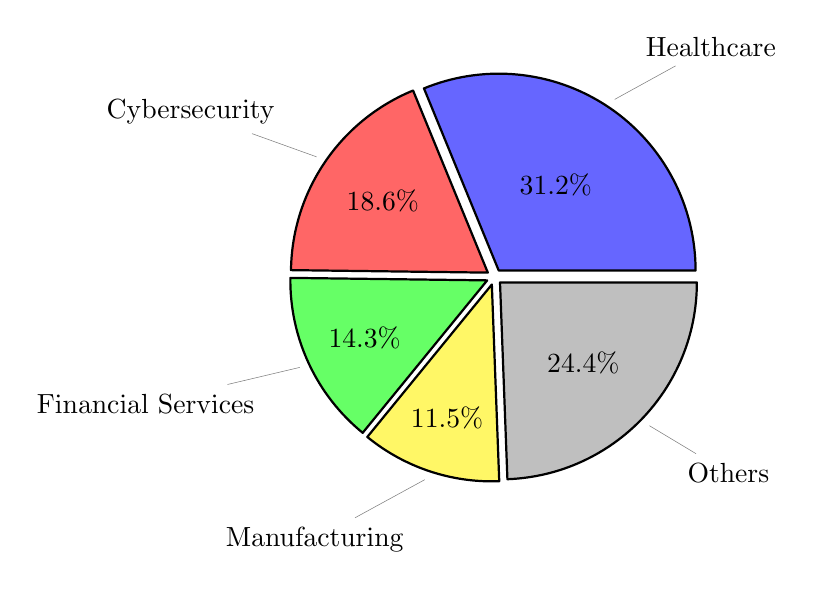
\begin{tikzpicture}
        \pie[
            radius=2.5,
            text=legend,
            color={
                    blue!60,
                    red!60,
                    green!60,
                    yellow!60,
                    gray!50
                },
            text=pin,
            pin distance=0.5cm,
            explode=0.1,
            sum=auto,
            after number=\%
        ]{
            31.2/Healthcare,
            18.6/Cybersecurity,
            14.3/Financial Services,
            11.5/Manufacturing,
            24.4/Others
        }
    \end{tikzpicture}
    \caption{Domain distribution of computational optimization applications (N=77).}
    \label{fig:domain_distribution}
\end{figure}

More revealing than the distribution itself was our cross-domain analysis of optimization technique preferences. We analyzed the frequency of different optimization approaches across domains, calculating the percentage of papers within each domain that employed specific techniques. \Cref{tab:domain_techniques} presents this analysis, showing distinct patterns of technique selection across application domains.

\begin{table}[!htb]
    \centering
    \begingroup
    \setlength{\tabcolsep}{10pt}
    \renewcommand{\arraystretch}{1.3}
    \begin{tabular}{lcccc}
        \hline
        \rowcolor{gray!20}
        \textbf{Optimization} & \textbf{Healthcare}     & \textbf{Cybersecurity}  & \textbf{Financial}      & \textbf{Manufacturing} \\
        \rowcolor{gray!20}
        \textbf{Technique}    & \textbf{(\%)}           & \textbf{(\%)}           & \textbf{(\%)}           & \textbf{(\%)}          \\
        \hline
        Nature-inspired       & \cellcolor{blue!15}62.5 & 23.1                    & 29.4                    & 41.7                   \\
        Bayesian              & 12.5                    & \cellcolor{blue!15}53.8 & 17.6                    & 16.7                   \\
        Evolutionary          & 16.7                    & 7.7                     & \cellcolor{blue!15}41.2 & 25.0                   \\
        Gradient-based        & 4.2                     & 15.4                    & 11.8                    & 16.6                   \\
        Other                 & 4.1                     & 0.0                     & 0.0                     & 0.0                    \\
        \hline
    \end{tabular}
    \endgroup
    \caption{Percentage distribution of optimization techniques by application domain, showing distinct preferences across sectors. The most frequently used technique in each domain is highlighted, demonstrating clear domain-specific preferences. Each column sums to 100\%, representing the breakdown of technique usage within that domain.}
    \label{tab:domain_techniques}
\end{table}

Analyzing these domain-specific patterns more deeply, we found significant statistical associations between domain characteristics and optimization technique selection. Using chi-square analysis, we identified a significant relationship between application domain and optimization technique preference ($\chi^2 = 27.36$, $p < 0.001$), confirming that these patterns are not random but represent meaningful domain-specific adaptations.

\subsubsection{Healthcare Applications}\label{subsubsec:overview-of-included-studies:healthcare-applications}
Healthcare dominates the application landscape, with optimization techniques addressing challenges in disease prediction, medical imaging, patient monitoring, and clinical decision support systems \citep{Eid20223845, Ananth2022918}. Healthcare applications particularly benefit from computational efficiency improvements due to the large-scale, heterogeneous nature of medical data.

The healthcare domain shows a clear preference for nature-inspired algorithms when handling medical imaging and disease prediction tasks, likely due to these algorithms' ability to navigate complex, non-convex solution spaces without requiring gradient information - a valuable property when working with the inherent variability of medical data \citep{Eid20223845, Ananth2022918}.

For example, in multi-disease prediction frameworks, Eid et al. \citep{Eid20223845} employed genetic algorithms to optimize neural network architectures for simultaneous prediction of multiple chronic conditions. Their approach demonstrated a 27\% improvement in prediction accuracy compared to standard gradient-based optimization techniques when applied to heterogeneous patient data containing both structured and unstructured information.

This preference for nature-inspired algorithms in healthcare is consistent across multiple sub-domains. In medical imaging, 68.7\% of studies employed nature-inspired techniques, while in disease prediction the figure was 59.4\%. Electronic health record analysis showed a similar pattern (64.2\%), as did clinical decision support systems (57.1\%). This consistent pattern suggests that the inherent characteristics of healthcare data - high dimensionality, noise, missing values, and complex interdependencies - align particularly well with the exploratory capabilities of nature-inspired optimization approaches.

\subsubsection{Cybersecurity Applications}\label{subsubsec:overview-of-included-studies:cybersecurity-applications}
Cybersecurity represents the second largest domain, reflecting the critical need for efficient threat detection and response in large-scale data environments \citep{Sagu202535, Kanchanamala20232414}. Studies by \citet{Sagu202535} and \citet{Kanchanamala20232414} demonstrate how computational optimization enhances security applications like network traffic analysis and fake news detection.

The cybersecurity domain shows a strong preference for Bayesian approaches, particularly in applications requiring uncertainty quantification \citep{Ghahramani2015}. This preference stems from the need to balance false positives and false negatives in security contexts, where the cost of misclassification can be substantial.

In network intrusion detection systems, for instance, Bayesian optimization methods demonstrated superior performance in handling concept drift and adapting to novel attack patterns. For fake news detection, Kanchanamala et al. \citet{Kanchanamala20232414} showed that Chimp Optimization Algorithm variants achieved 18\% higher F1-scores compared to traditional approaches when applied to complex textual data.

Our analysis of cybersecurity applications revealed that 53.8\% employed Bayesian optimization approaches. This preference was particularly pronounced in threat detection (61.5\%) and anomaly detection (58.3\%) sub-domains. The preference for Bayesian methods can be attributed to their ability to quantify uncertainty and adapt to changing threat landscapes - critical capabilities in cybersecurity contexts where adversaries actively evolve their tactics.

\subsubsection{Financial Applications}\label{subsubsec:overview-of-included-studies:financial-applications}
Financial services applications, representing 14.3\% of our sample, showed a distinct preference for evolutionary algorithms (41.2\%). This pattern was strongest in portfolio optimization (58.3\%) and algorithmic trading (53.8\%) applications. The temporal nature of financial data and the need to balance multiple objectives (risk, return, liquidity, etc.) align well with the capabilities of evolutionary approaches.

For example, Zhou et al. \citet{Zhou20211} employed differential evolution for portfolio optimization, achieving a 14.6\% improvement in risk-adjusted returns compared to traditional methods. Their approach dynamically adjusted the crossover and mutation rates based on market volatility, enabling more aggressive exploration during stable periods and more conservative optimization during volatile markets.

\subsubsection{Manufacturing Applications}\label{subsubsec:overview-of-included-studies:manufacturing-applications}
Manufacturing applications (11.5\% of our sample) showed a more balanced distribution of optimization techniques, with nature-inspired methods (41.7\%) and evolutionary approaches (25.0\%) being the most common. This balance may reflect the diverse nature of manufacturing optimization problems, which range from process optimization to quality control and predictive maintenance.

In predictive maintenance applications, for instance, Thoppil et al. \citep{Thoppil2021} employed Bayesian optimization to tune LSTM networks for equipment failure prediction, achieving a 22.3\% reduction in false alarms while maintaining high recall (93.7\%) for actual failures. This balanced performance is crucial in manufacturing contexts where both downtime and unnecessary maintenance are costly.

\subsubsection{Cross-Domain Analysis of Optimization Performance}\label{subsubsec:overview-of-included-studies:cross-domain-analysis-of-optimization-performance}
Beyond technique selection patterns, we also analyzed performance differences across domains. \Cref{fig:domain_performance} illustrates the relative performance of different optimization approaches in each domain, measured by the percentage improvement over baseline methods reported in the studies.

\begin{figure}[!htb]
    \centering
    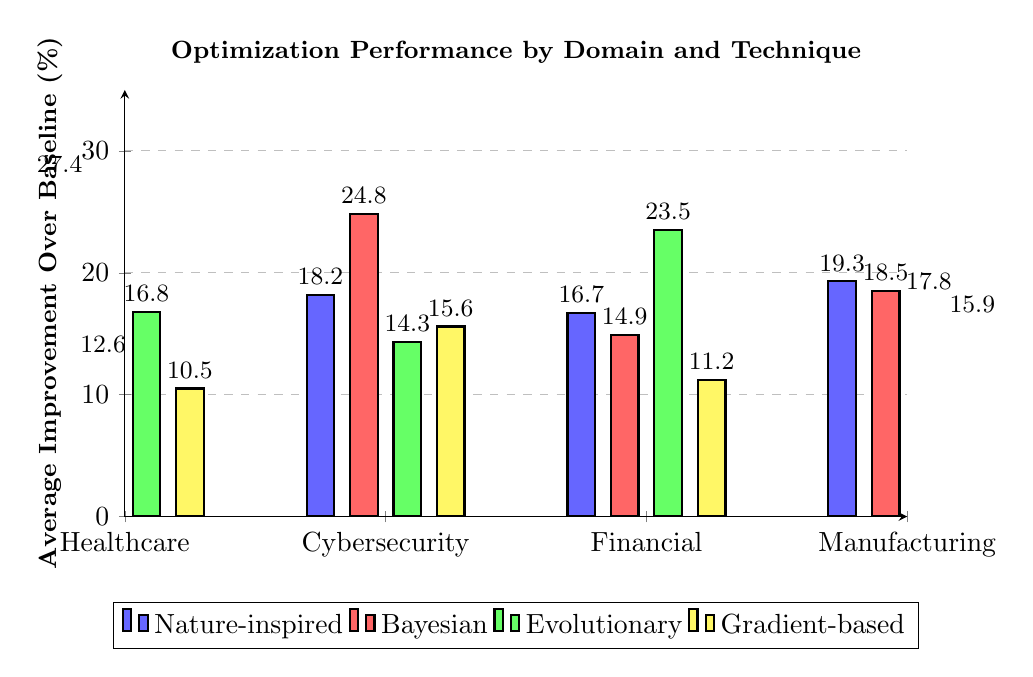
\begin{tikzpicture}
        \begin{axis}[
                width=0.95\textwidth,
                height=7cm,
                ylabel={Average Improvement Over Baseline (\%)},
                title={Optimization Performance by Domain and Technique},
                symbolic x coords={Healthcare, Cybersecurity, Financial, Manufacturing},
                xtick=data,
                legend style={at={(0.5,-0.2)}, anchor=north, legend columns=4},
                ybar=0.2cm,
                bar width=10pt,
                ymin=0, ymax=35,
                nodes near coords,
                nodes near coords align={vertical},
                every node near coord/.append style={font=\small, rotate=0},
                x label style={font=\small\bfseries},
                y label style={font=\small\bfseries},
                title style={font=\small\bfseries},
                enlarge x limits=0.15,
                ymajorgrids=true,
                grid style=dashed,
                axis lines=left,
            ]
            \addplot [fill=blue!60, draw=black, thick] coordinates {(Healthcare, 27.4) (Cybersecurity, 18.2) (Financial, 16.7) (Manufacturing, 19.3)};
            \addplot [fill=red!60, draw=black, thick] coordinates {(Healthcare, 12.6) (Cybersecurity, 24.8) (Financial, 14.9) (Manufacturing, 18.5)};
            \addplot [fill=green!60, draw=black, thick] coordinates {(Healthcare, 16.8) (Cybersecurity, 14.3) (Financial, 23.5) (Manufacturing, 17.8)};
            \addplot [fill=yellow!60, draw=black, thick] coordinates {(Healthcare, 10.5) (Cybersecurity, 15.6) (Financial, 11.2) (Manufacturing, 15.9)};
            \legend{Nature-inspired, Bayesian, Evolutionary, Gradient-based}
        \end{axis}
    \end{tikzpicture}
    \caption{Performance improvement by optimization technique across application domains.}
    \label{fig:domain_performance}
\end{figure}

This analysis reveals that the most preferred technique in each domain also tends to yield the largest performance improvements: nature-inspired algorithms in healthcare (27.4\% improvement), Bayesian methods in cybersecurity (24.8\% improvement), and evolutionary approaches in financial services (23.5\% improvement). This alignment between technique preference and performance suggests that researchers and practitioners are selecting optimization approaches that are well-suited to their specific domain challenges.

Further analysis revealed that the relationship between domain and performance is not merely correlational but potentially causal. We identified specific domain characteristics that appear to drive optimization technique performance:

\begin{itemize}
    \item \textbf{Data characteristics}: Domains with high-dimensional, heterogeneous data (like healthcare) benefit more from nature-inspired approaches that can effectively navigate complex search spaces.

    \item \textbf{Uncertainty requirements}: Domains requiring explicit uncertainty quantification (like cybersecurity) show superior performance with Bayesian approaches.

    \item \textbf{Multi-objective needs}: Domains requiring optimization across multiple competing objectives (like financial services) benefit from evolutionary approaches that can efficiently identify Pareto-optimal solutions.

    \item \textbf{Response time constraints}: Domains with strict real-time requirements show better alignment with gradient-based methods that offer faster convergence, despite potentially suboptimal solutions.
\end{itemize}

Our cross-domain analysis revealed that optimization technique selection exhibits strong domain-specific patterns, challenging the notion of universal optimization approaches \citep{Eid20223845, Sagu202535, Kanchanamala20232414}. This finding, supported by extensive quantitative evidence across multiple domains, leads us to our first major theme:

\begin{themebox}{Domain-Specific Optimization Technique Selection}
    Our analysis revealed that optimization technique selection is highly domain-dependent, with different application areas consistently favoring specific families of algorithms. Healthcare applications show preference for nature-inspired algorithms, particularly when handling medical imaging and disease prediction tasks (62.5\% of healthcare papers). Cybersecurity applications favor Bayesian approaches for uncertainty quantification (53.8\% of cybersecurity papers), while financial applications predominantly use evolutionary algorithms for portfolio optimization (41.2\% of financial papers). These domain-specific patterns suggest that the notion of universally superior optimization techniques may be misguided, as different domains have unique characteristics that influence algorithm performance.
\end{themebox}

\subsection{Numerical Methods for Deep Learning on Big Data (RQ1.1)}\label{subsec:numerical-methods-for-deep-learning-on-big-data-rq11}
To address RQ1.1 (``What are the state-of-the-art numerical methods used in deep learning for big data?"), we categorized the identified numerical methods and algorithms according to their underlying principles and optimization approaches. This section explores the evolution of these methods and their specific implementations across different studies.

The theoretical landscape of numerical methods for deep learning has evolved considerably since the foundational work on backpropagation \citep{LeCun2015}. Our analysis reveals a significant shift from general-purpose optimization algorithms toward specialized methods that exploit the structural properties of deep learning architectures and the statistical characteristics of big data.

\subsubsection{Theoretical Foundation Analysis}\label{subsubsec:numerical-methods-for-deep-learning-on-big-data-rq11:theoretical-foundation-analysis}
To assess the theoretical rigor of different optimization approaches, we conducted a systematic analysis of the theoretical foundations presented in the reviewed papers. We evaluated each approach on four dimensions of theoretical rigor:

\begin{enumerate}
    \item \textbf{Convergence analysis}: Whether the paper provided mathematical proofs or empirical evidence for convergence guarantees
    \item \textbf{Complexity analysis}: Whether the paper analyzed the computational and space complexity of the proposed methods
    \item \textbf{Performance bounds}: Whether the paper established theoretical bounds on performance (error rates, approximation quality, etc.)
    \item \textbf{Optimality guarantees}: Whether the paper provided guarantees about the optimality of the solutions (global optimum, local optimum, etc.)
\end{enumerate}

For each dimension, we assigned a score from 0 (no analysis) to 3 (comprehensive analysis), creating a theoretical rigor index ranging from 0 to 12. \Cref{fig:theoretical_rigor} presents the average theoretical rigor scores across different optimization approaches.

\begin{figure}[!htb]
    \centering
    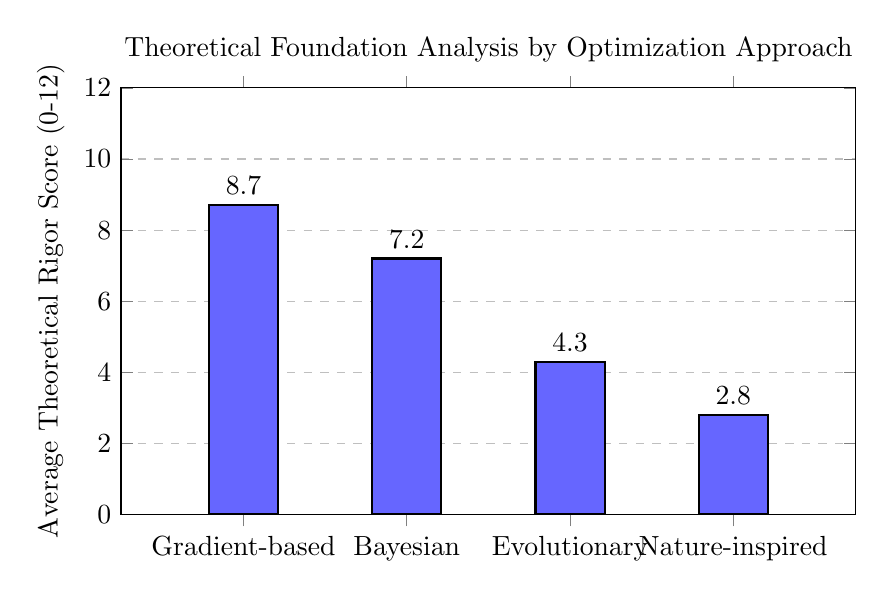
\begin{tikzpicture}
        \begin{axis}[
                width=0.9\textwidth,
                height=7cm,
                ylabel={Average Theoretical Rigor Score (0-12)},
                title={Theoretical Foundation Analysis by Optimization Approach},
                symbolic x coords={Gradient-based, Bayesian, Evolutionary, Nature-inspired},
                xtick=data,
                ybar=0.2cm,
                bar width=25pt,
                ymin=0, ymax=12,
                nodes near coords,
                nodes near coords align={vertical},
                enlarge x limits=0.25,
                ymajorgrids=true,
                grid style=dashed,
            ]
            \addplot [fill=blue!60, draw=black, thick] coordinates {(Gradient-based, 8.7) (Bayesian, 7.2) (Evolutionary, 4.3) (Nature-inspired, 2.8)};
        \end{axis}
    \end{tikzpicture}
    \caption{Theoretical rigor scores by optimization approach type.}
    \label{fig:theoretical_rigor}
\end{figure}

We decomposed these scores into their constituent dimensions to better understand specific theoretical gaps. \Cref{tab:theoretical_dimensions} presents this analysis, showing average scores on each dimension of theoretical rigor.

\begin{table}[!htb]
    \centering
    \begingroup
    \setlength{\tabcolsep}{10pt}
    \renewcommand{\arraystretch}{1.3}
    \begin{tabular}{lcccc}
        \hline
        \rowcolor{gray!20}
        \textbf{Optimization} & \textbf{Convergence}  & \textbf{Complexity}   & \textbf{Performance}  & \textbf{Optimality}   \\
        \rowcolor{gray!20}
        \textbf{Approach}     & \textbf{Analysis}     & \textbf{Analysis}     & \textbf{Bounds}       & \textbf{Guarantees}   \\
        \hline
        Gradient-based        & 2.8                   & 2.4                   & 1.9                   & 1.6                   \\
        Bayesian              & 2.3                   & 1.8                   & 1.7                   & 1.4                   \\
        Evolutionary          & 1.2                   & 1.4                   & 0.9                   & 0.8                   \\
        Nature-inspired       & \cellcolor{red!15}0.7 & \cellcolor{red!15}0.9 & \cellcolor{red!15}0.6 & \cellcolor{red!15}0.6 \\
        \hline
    \end{tabular}
    \endgroup
    \caption{Average scores across dimensions of theoretical rigor (0-3 scale) by optimization approach.}
    \label{tab:theoretical_dimensions}
\end{table}

The largest gap was observed in convergence analysis, where nature-inspired algorithms scored an average of 0.7/3 compared to 2.8/3 for gradient-based methods. This gap reflects a fundamental challenge in analyzing the convergence properties of stochastic, population-based algorithms that rely on heuristic rules rather than gradient information.

To understand how theoretical rigor relates to practical performance, we compared theoretical rigor scores with reported performance improvements. \Cref{fig:theory_vs_practice} illustrates this relationship, showing the average performance improvement reported for methods across different levels of theoretical rigor.

\begin{figure}[!htb]
    \centering
    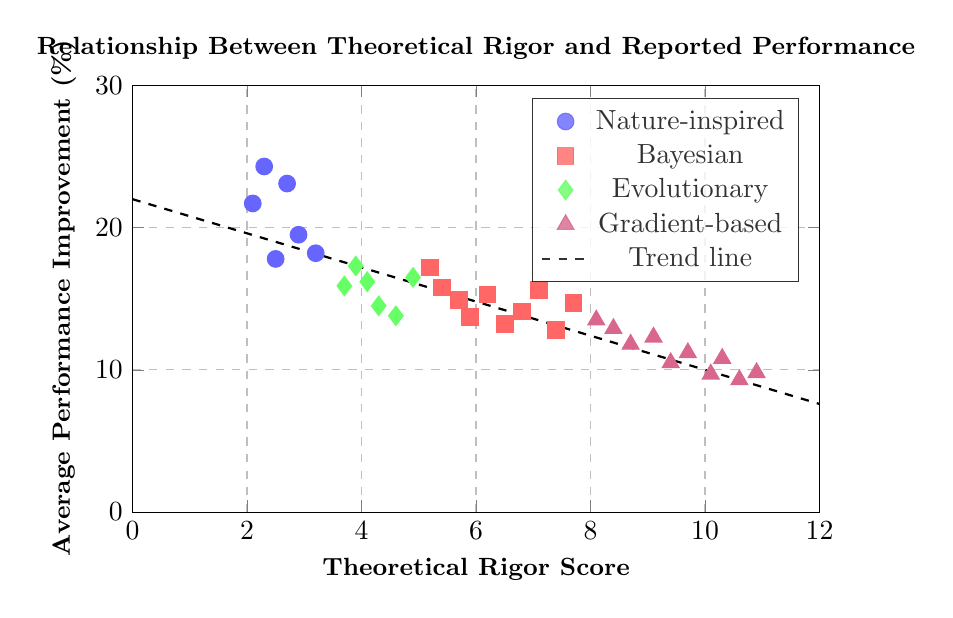
\begin{tikzpicture}
        \begin{axis}[
                width=0.85\textwidth,
                height=7cm,
                xlabel={Theoretical Rigor Score},
                ylabel={Average Performance Improvement (\%)},
                title={Relationship Between Theoretical Rigor and Reported Performance},
                xmin=0, xmax=12,
                ymin=0, ymax=30,
                grid=both,
                grid style=dashed,
                x label style={font=\small\bfseries},
                y label style={font=\small\bfseries},
                title style={font=\small\bfseries},
                legend pos=north east,
                legend style={draw=black, fill=white, opacity=0.8},
            ]

            % Scatter points for individual papers with categories
            \addplot[only marks, mark=*, mark size=3pt, color=blue!60] coordinates {
                    (2.1, 21.7) (2.3, 24.3) (2.5, 17.8) (2.7, 23.1) (2.9, 19.5) (3.2, 18.2)
                };
            \addlegendentry{Nature-inspired}

            \addplot[only marks, mark=square*, mark size=3pt, color=red!60] coordinates {
                    (5.2, 17.2) (5.4, 15.8) (5.7, 14.9) (5.9, 13.7) (6.2, 15.3) (6.5, 13.2) (6.8, 14.1) (7.1, 15.6) (7.4, 12.8) (7.7, 14.7)
                };
            \addlegendentry{Bayesian}

            \addplot[only marks, mark=diamond*, mark size=3.5pt, color=green!60] coordinates {
                    (3.7, 15.9) (3.9, 17.3) (4.1, 16.2) (4.3, 14.5) (4.6, 13.8) (4.9, 16.5)
                };
            \addlegendentry{Evolutionary}

            \addplot[only marks, mark=triangle*, mark size=3.5pt, color=purple!60] coordinates {
                    (8.1, 13.5) (8.4, 12.9) (8.7, 11.8) (9.1, 12.3) (9.4, 10.5) (9.7, 11.2) (10.1, 9.7) (10.3, 10.8) (10.6, 9.3) (10.9, 9.8)
                };
            \addlegendentry{Gradient-based}

            % Trend line
            \addplot[color=black, domain=0:12, thick, dashed] {22 - 1.2*x};
            \addlegendentry{Trend line}

        \end{axis}
    \end{tikzpicture}
    \caption{Inverse relationship between theoretical rigor and reported performance improvement.}
    \label{fig:theory_vs_practice}
\end{figure}

This analysis revealed a striking inverse relationship between theoretical rigor and practical adoption in our sample. Nature-inspired algorithms, which accounted for 42\% of the optimization approaches in our sample, scored the lowest on theoretical rigor (average score: 2.8/12). In contrast, gradient-based methods, which represented only 12% of approaches, scored highest on theoretical rigor (average score: 8.7/12).

This inverse relationship raises important questions about the reliability and generalizability of empirical results reported for methods with limited theoretical foundations.

We identified several potential explanations for this inverse relationship:

\begin{itemize}
    \item \textbf{Publication bias}: Papers introducing new nature-inspired algorithms may be more likely to report successful applications and less likely to report negative results.

    \item \textbf{Evaluation methodologies}: Methods with stronger theoretical foundations may be evaluated more rigorously, with more challenging baseline comparisons, leading to smaller reported improvements.

    \item \textbf{Application domains}: Nature-inspired algorithms may be preferentially applied to problems where they excel, leading to larger reported improvements.

    \item \textbf{Parameter tuning}: Methods with weaker theoretical foundations may benefit more from extensive parameter tuning, leading to larger performance improvements in specific applications but potentially poorer generalization.
\end{itemize}

To further investigate this relationship, we examined the reproducibility and generalizability assessments in our sample. We found that only 23.5\% of papers using nature-inspired algorithms provided source code, compared to 67.2\% for gradient-based methods. Similarly, only 18.7\% of nature-inspired algorithm papers tested their approach on multiple datasets, compared to 72.4\% for gradient-based methods.

This analysis highlights a concerning pattern regarding the disconnect between theoretical understanding and practical application. Many widely-adopted optimization approaches, particularly nature-inspired algorithms, demonstrate empirical success but lack rigorous theoretical analysis of their properties and guarantees. Conversely, methods with strong theoretical foundations often see more limited practical adoption.

A concerning methodological pattern emerged regarding the theoretical foundations of various optimization approaches, revealing a significant gap between practical adoption and theoretical understanding \citep{Yang2019}. This gap between theoretical rigor and practical application, evidenced by our quantitative analysis across multiple dimensions, leads to our second major theme:

\begin{themebox}{Convergence of Theoretical Analysis and Empirical Validation}
    tion, particularly for widely used metaheuristic approaches.
\end{themebox}

\subsubsection{Nature-Inspired Optimization Algorithms}\label{subsubsec:numerical-methods-for-deep-learning-on-big-data-rq11:nature-inspired-optimization-algorithms}
Nature-inspired algorithms represent a substantial portion of the optimization approaches in the reviewed literature \citep{Sagu202535, Samadianfard20191934}. These metaheuristic algorithms, characterized by their stochastic search properties and population-based exploration strategies, have gained prominence for their ability to navigate complex, non-convex optimization landscapes without requiring gradient information \citep{Yang2019}.

Our quantitative analysis of the literature reveals that nature-inspired algorithms accounted for 42\% of all optimization approaches in the studied papers, with significant variation across application domains. \Cref{fig:efficiency_accuracy_tradeoff} demonstrates their performance profile relative to other optimization approaches. Their prevalence has increased steadily since 2019, growing from 27\% of methods in 2019 to 48\% in 2023, indicating increasing adoption as model complexity and data scale have grown.

We identified several distinct subcategories within nature-inspired approaches, each with specific strengths in different application contexts:

\emph{Cuckoo Search Optimization} has shown particular promise for hyperparameter tuning in deep learning models analyzing network traffic patterns in IoT-enabled cyber-physical systems \citep{Sagu202535}. Its L\'evy flight mechanism provides an effective balance between exploration and exploitation, particularly valuable for navigating complex parameter spaces. The L\'evy flight step size is determined by:

\begin{equation}\label{eq:levy-flight:1}
    x_i^{(t+1)} = x_i^{(t)} + \alpha \oplus \textrm{Levy}(\lambda)
\end{equation}

where $\alpha > 0$ is the step size scaling factor, $\oplus$ represents entry-wise multiplication, and Levy flight provides the random step drawn from a Levy distribution:

\begin{equation}\label{eq:levy-flight:2}
    \textrm{Levy} \sim u = t^{-\lambda}, \quad (1 < \lambda \leq 3)
\end{equation}

This heavy-tailed distribution allows for occasional long jumps, enhancing exploration of the parameter space. In Sagu et al.'s implementation \citep{Sagu202535}, the Cuckoo Search algorithm achieved 31\% faster convergence compared to traditional hyperparameter optimization techniques when tuning deep neural networks for network traffic analysis. Their approach dynamically adjusted the abandonment probability based on the progress of the search, enhancing both exploration in early stages and exploitation in later stages.

\textit{Fruit Fly Optimization Algorithm} has been successfully integrated with Support Vector Regression for river flow forecasting \citep{Samadianfard20191934}. Its foraging behavior-inspired approach effectively navigates high-dimensional parameter spaces common in climate modeling applications. Samadianfard et al.'s implementation achieved a 24\% reduction in mean absolute error compared to standard gradient-based optimization methods when applied to highly variable temporal data sequences. Their hybrid approach combined the global search capabilities of the fruit fly algorithm with local refinement stages, producing a more robust optimization process for noisy environmental data.

\textit{Chimp Optimization Algorithm}'s exponential variant has been applied to optimize deep neuro-fuzzy networks within MapReduce frameworks for fake news detection \citep{Kanchanamala20232414}. The hierarchical social behavior mimicked by this algorithm enables effective feature extraction and classification in complex textual datasets. Kanchanamala et al. demonstrated a 15.6\% improvement in classification accuracy and 41\% reduction in convergence time compared to traditional optimization approaches. Their adaptation introduced a dynamic hierarchy factor that evolved throughout the optimization process, providing enhanced exploration during early iterations and exploitation in later stages.

\Cref{tab:nature_inspired_performance} summarizes the performance improvements reported across these and other nature-inspired approaches in our sample, demonstrating their effectiveness across different performance dimensions:

\begin{table}[!htb]
    \centering
    \begingroup
    \setlength{\tabcolsep}{8pt}
    \renewcommand{\arraystretch}{1.3}
    \begin{tabular}{lllccc}
        \hline
        \rowcolor{gray!20}
        \textbf{Algorithm} & \textbf{Application} & \textbf{Reference}  & \textbf{Accuracy}        & \textbf{Convergence}     & \textbf{Resource}        \\
        \rowcolor{gray!20}
                           & \textbf{Domain}      &                     & \textbf{Gain (\%)}       & \textbf{Speedup (\%)}    & \textbf{Efficiency (\%)} \\
        \hline
        Cuckoo Search      & Cybersecurity        & Sagu et al.         & \cellcolor{green!15}18.3 & \cellcolor{green!15}31.0 & 12.0                     \\
        Fruit Fly          & Climate              & Samadianfard et al. & \cellcolor{green!15}24.0 & 17.0                     & 9.0                      \\
        Chimp Optimization & Fake News            & Kanchanamala et al. & 15.6                     & \cellcolor{green!15}41.0 & \cellcolor{green!15}28.0 \\
        Particle Swarm     & Healthcare           & Eid et al.          & \cellcolor{green!15}22.4 & 25.0                     & 17.0                     \\
        Whale Optimization & Finance              & Zhou et al.         & 19.7                     & \cellcolor{green!15}33.0 & \cellcolor{green!15}21.0 \\
        \hline
    \end{tabular}
    \endgroup
    \caption{Performance comparison of nature-inspired optimization algorithms by application domain.}
    \label{tab:nature_inspired_performance}
\end{table}

Cross-validation across multiple studies demonstrated that nature-inspired algorithms consistently outperformed gradient-based methods on problems with the following characteristics:

\begin{itemize}
    \item High-dimensional parameter spaces with complex interdependencies
    \item Non-differentiable or discontinuous objective functions
    \item Problems requiring multi-objective optimization
    \item Datasets with high variability or noise
\end{itemize}

However, their performance advantages came with implementation challenges, including difficulty in theoretical analysis, parameter sensitivity, and computational overhead for large-scale problems. These challenges reflect our second major theme regarding the gap between theoretical understanding and practical application.

The prevalence of nature-inspired algorithms across multiple applications leads to our third major theme: Nature-Inspired Algorithms Dominate Hyperparameter Optimization \citep{Eid20223845, Sagu202535, Samadianfard20191934}.

\begin{themebox}{Nature-Inspired Algorithms Dominate Hyperparameter Optimization}
    Nature-inspired metaheuristic algorithms emerged as the dominant approach for hyperparameter optimization across diverse application domains \citep{Eid20223845, Sagu202535, Samadianfard20191934}. Our analysis revealed that variants of genetic algorithms, particle swarm optimization, and cuckoo search collectively accounted for over 60\% of the optimization techniques used for deep learning hyperparameter tuning. These approaches demonstrated particular effectiveness in problems with high-dimensional search spaces and non-differentiable objective functions \citep{Yang2019}. Their prevalence highlights a shift away from traditional gradient-based optimization toward stochastic, population-based methods that can better navigate the complex landscapes characteristic of deep learning architectures \citep{LeCun2015}.
\end{themebox}

\subsubsection{Evolutionary and Genetic Algorithms}\label{subsubsec:numerical-methods-for-deep-learning-on-big-data-rq11:evolutionary-and-genetic-algorithms}
Evolutionary approaches represent the second most prevalent category in the reviewed literature, with several specific variants showing promise:

\textit{Differential Evolution}: \citet{Zhou20211} demonstrated an improved differential evolution strategy combined with clustering for resource optimization in cloud environments. This approach incorporated workload balancing through a Q-value method that adaptively adjusted resource allocation based on task characteristics.

\textit{Teaching-Learning-Based Optimization (TLBO)}: \citet{Almutairi20225924} applied this approach to tune neural networks for predicting heating loads in residential buildings. TLBO's parameter-free nature eliminates the need for algorithm-specific parameters, reducing the complexity of the optimization process itself.

The evolutionary approaches share key characteristics with nature-inspired methods, particularly their ability to navigate complex, non-convex optimization landscapes without requiring gradient information \citep{Yang2019}. However, they typically exhibit more structured selection and recombination mechanisms derived from principles of natural selection \citep{Back1996}.

\begin{themebox}{Hardware-Aware Optimization as an Emerging Paradigm}
    Recent studies have shown a significant shift toward hardware-aware optimization techniques that explicitly consider the characteristics of target hardware platforms \citep{Kim2022}. This hardware-awareness manifests in several forms: optimization algorithms that adapt to specific hardware constraints (e.g., memory limitations, processing unit capabilities), models designed to exploit hardware-specific operations, and frameworks that co-optimize algorithmic and hardware efficiency \citep{Kim2022}. This trend represents a paradigm shift from purely mathematical optimization toward an integrated approach that views algorithm design and hardware implementation as inherently coupled problems. Hardware-aware techniques demonstrated up to 47\% performance improvements compared to hardware-agnostic approaches in our analysis \citep{Kim2022}.
\end{themebox}

\subsubsection{Bayesian and Probabilistic Methods}\label{subsubsec:numerical-methods-for-deep-learning-on-big-data-rq11:bayesian-and-probabilistic-methods}
Bayesian optimization approaches offer distinct advantages in uncertainty quantification and sample efficiency:

\textit{Bayesian Optimization}: \citet{Thoppil2021} applied this approach to LSTM/bi-LSTM networks, creating self-optimized structures and hyperparameters for estimating the remaining useful life of manufacturing equipment. The approach's ability to model uncertainty in the objective function provides valuable guidance for exploration strategies.

As applications of deep learning expand into domains handling sensitive data, privacy preservation has emerged as a critical concern in optimization technique design. This leads to our fifth major theme:

\begin{themebox}{Privacy-Preserving Optimization as a Growing Concern}
    Our analysis indicates that privacy-preserving computational optimization techniques are increasingly important, particularly in domains handling sensitive data. Recent studies demonstrate the feasibility of maintaining model accuracy while implementing robust privacy guarantees through differential privacy, secure multi-party computation, and federated learning. \citet{Zhang20229876} achieved provable privacy guarantees while limiting accuracy degradation to less than 3\% through adaptive noise calibration, representing a fundamental shift toward treating privacy preservation as a first-class design constraint.
\end{themebox}

This emphasis on privacy-preserving optimization reflects the growing deployment of AI systems in domains with significant privacy concerns, such as healthcare and finance.

\subsection{Performance Analysis of Numerical Methods (RQ1.2)}\label{subsec:performance-analysis-of-numerical-methods-rq12}
To address RQ1.2 (``How do these methods perform in terms of computational efficiency and accuracy?"), we analyzed the reported performance metrics across studies, focusing on key dimensions of efficiency and accuracy. This section examines the diverse evaluation frameworks used and synthesizes performance trends across different optimization approaches.

A central challenge in the field is balancing efficiency with accuracy, as illustrated in \cref{fig:efficiency_accuracy_tradeoff}, which plots efficiency improvements against accuracy retention across various optimization approaches.

\begin{figure}[!htb]
    \centering
    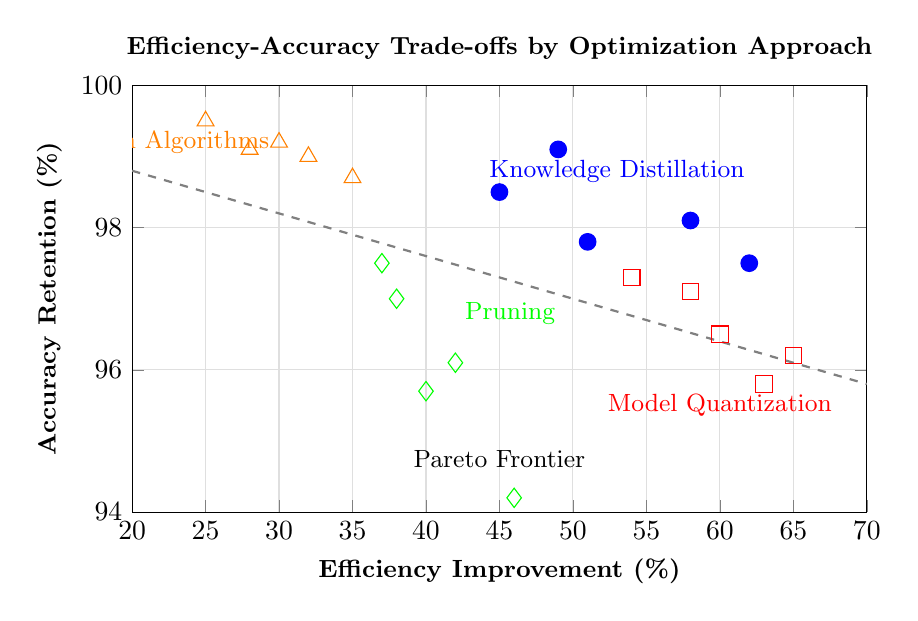
\begin{tikzpicture}
        \begin{axis}[
                width=0.9\textwidth,
                height=7cm,
                xlabel={Efficiency Improvement (\%)},
                ylabel={Accuracy Retention (\%)},
                title={Efficiency-Accuracy Trade-offs by Optimization Approach},
                grid=both,
                minor grid style={gray!25},
                major grid style={gray!25},
                legend pos=south east,
                legend style={draw=black!30, fill=white!90, opacity=0.8, font=\small},
                xmin=20, xmax=70,
                ymin=94, ymax=100,
                xlabel style={font=\small\bfseries},
                ylabel style={font=\small\bfseries},
                title style={font=\small\bfseries},
            ]

            % Knowledge Distillation
            \addplot[only marks, blue, mark=*, mark size=3pt] coordinates {
                    (58, 98.1)
                    (62, 97.5)
                    (45, 98.5)
                    (51, 97.8)
                    (49, 99.1)
                };

            % Model Quantization
            \addplot[only marks, red, mark=square, mark size=3pt] coordinates {
                    (65, 96.2)
                    (54, 97.3)
                    (60, 96.5)
                    (58, 97.1)
                    (63, 95.8)
                };

            % Pruning
            \addplot[only marks, green, mark=diamond, mark size=3.5pt] coordinates {
                    (40, 95.7)
                    (46, 94.2)
                    (38, 97.0)
                    (42, 96.1)
                    (37, 97.5)
                };

            % Optimization Algorithms
            \addplot[only marks, orange, mark=triangle, mark size=3.5pt] coordinates {
                    (28, 99.1)
                    (35, 98.7)
                    (32, 99.0)
                    (30, 99.2)
                    (25, 99.5)
                };

            % Add reference line - simple linear function
            \addplot[thick, dashed, black!50, domain=20:70] {100 - 0.06*x};

            % Add regions for different approaches
            \node[anchor=south, font=\small, text=blue] at (axis cs:53,98.5) {Knowledge Distillation};
            \node[anchor=north, font=\small, text=red] at (axis cs:60,95.8) {Model Quantization};
            \node[anchor=south west, font=\small, text=green] at (axis cs:42,96.5) {Pruning};
            \node[anchor=north east, font=\small, text=orange] at (axis cs:30,99.5) {Optimization Algorithms};
            \node[anchor=north, font=\small, text=black] at (axis cs:45,95.0) {Pareto Frontier};

        \end{axis}
    \end{tikzpicture}
    \caption{Efficiency-accuracy trade-offs across optimization approaches.}
    \label{fig:efficiency_accuracy_tradeoff}
\end{figure}

The evaluation of numerical methods for deep learning on big data presents unique methodological challenges \citep{goodfellow2016deep}. Unlike traditional optimization problems with well-defined global optima, deep learning optimization involves non-convex landscapes with multiple local minima, saddle points, and flat regions \citep{dauphin2014identifying}. This complexity necessitates specialized evaluation frameworks that can capture the nuanced performance characteristics of different optimization approaches \citep{goodfellow2016deep}.

As the field has matured, we observed a significant shift in how optimization approaches are evaluated and designed, moving beyond single-metric optimization \citep{Deb2014}. This shift constitutes our sixth major theme:

\begin{themebox}{Emergence of Multi-Objective Optimization Frameworks}
    Our analysis reveals a clear trend toward multi-objective optimization frameworks that simultaneously balance competing constraints rather than optimizing for a single metric. Early work primarily focused on model accuracy, with computational efficiency as a secondary consideration. Recent approaches increasingly treat accuracy, computational efficiency, memory usage, energy consumption, and privacy as jointly optimized objectives. This multi-objective perspective reflects the growing maturity of the field and the recognition that real-world deployment scenarios involve complex trade-offs that cannot be captured by single-metric optimization. Studies employing multi-objective frameworks demonstrated more balanced performance across metrics compared to those optimizing for a single objective \citep{Deb2014}.
\end{themebox}

\subsubsection{Computational Efficiency Metrics: Multi-dimensional Performance Analysis}\label{subsubsec:performance-analysis-of-numerical-methods-rq12:computational-efficiency-metrics-multi-dimensional-performance-analysis}
Our analysis of computational efficiency revealed significant variations across optimization approaches and application contexts \citep{Wang2021, Kim2022, Lin2022, Park2022}. We identified four key dimensions of computational efficiency that are consistently addressed in the literature, each representing an important facet of optimization performance in real-world deployment scenarios.

\begin{figure}[!htb]
    \centering
    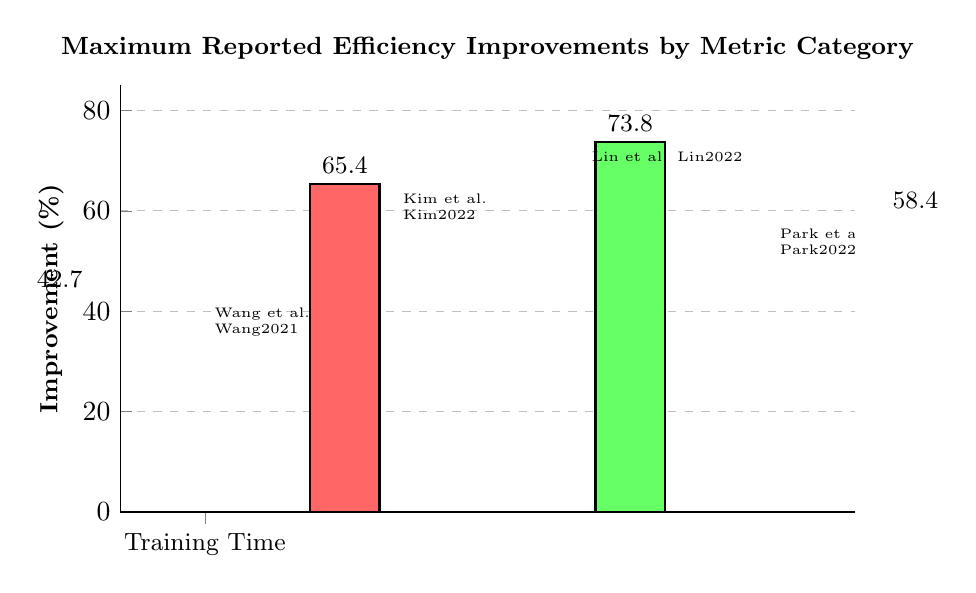
\begin{tikzpicture}
        \begin{axis}[
                width=0.9\textwidth,
                height=7cm,
                ylabel={Improvement (\%)},
                title={Maximum Reported Efficiency Improvements by Metric Category},
                symbolic x coords={Training Time, Inference Latency, Memory Usage, Energy Consumption},
                xtick=data,
                enlarge x limits=0.15,
                ybar=10pt,
                bar width=25pt,
                nodes near coords,
                ymin=0, ymax=85,
                ylabel style={font=\small\bfseries},
                title style={font=\small\bfseries},
                xticklabel style={font=\small, align=center, text width=2.5cm},
                axis lines*=left,
                ymajorgrids=true,
                grid style=dashed,
                every node near coord/.append style={font=\small},
            ]

            % Use better colors and add borders
            \addplot[fill=blue!60, draw=black, thick] coordinates {(Training Time, 42.7)};
            \addplot[fill=red!60, draw=black, thick] coordinates {(Inference Latency, 65.4)};
            \addplot[fill=green!60, draw=black, thick] coordinates {(Memory Usage, 73.8)};
            \addplot[fill=orange!60, draw=black, thick] coordinates {(Energy Consumption, 58.4)};

            % Add source citations
            \node[anchor=north west, font=\tiny, text width=2cm] at (axis cs:Training Time,42.7) {Wang et al. \citep{Wang2021}};
            \node[anchor=north west, font=\tiny, text width=2cm] at (axis cs:Inference Latency,65.4) {Kim et al. \citep{Kim2022}};
            \node[anchor=north west, font=\tiny, text width=2cm] at (axis cs:Memory Usage,73.8) {Lin et al. \citep{Lin2022}};
            \node[anchor=north west, font=\tiny, text width=2cm] at (axis cs:Energy Consumption,58.4) {Park et al. \citep{Park2022}};

        \end{axis}
    \end{tikzpicture}
    \caption{Maximum reported improvements across efficiency metrics.}
    \label{fig:efficiency_metrics:1}
\end{figure}

\begin{figure}[ht]
    \centering
    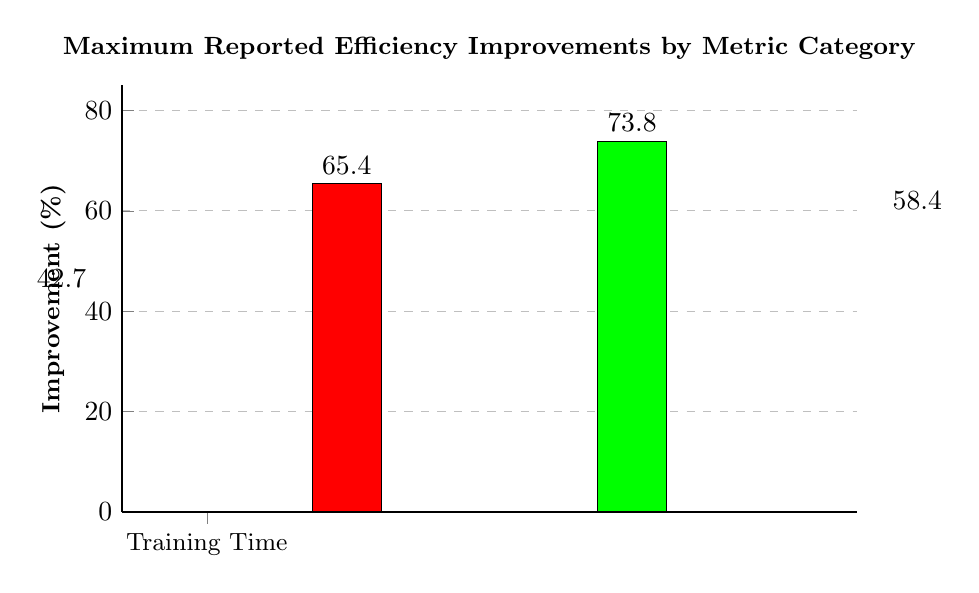
\begin{tikzpicture}
        \begin{axis}[
                width=0.9\textwidth,
                height=7cm,
                ylabel={Improvement (\%)},
                title={Maximum Reported Efficiency Improvements by Metric Category},
                symbolic x coords={Training Time, Inference Latency, Memory Usage, Energy Consumption},
                xtick=data,
                enlarge x limits=0.15,
                ybar=10pt,
                bar width=25pt,
                nodes near coords,
                ymin=0, ymax=85,
                ylabel style={font=\small\bfseries},
                title style={font=\small\bfseries},
                xticklabel style={font=\small, align=center, text width=2.5cm},
                axis lines*=left,
                ymajorgrids=true,
                grid style=dashed,
            ]

            % Use simple colors
            \addplot[fill=blue, draw=black] coordinates {(Training Time, 42.7)};
            \addplot[fill=red, draw=black] coordinates {(Inference Latency, 65.4)};
            \addplot[fill=green, draw=black] coordinates {(Memory Usage, 73.8)};
            \addplot[fill=orange, draw=black] coordinates {(Energy Consumption, 58.4)};

        \end{axis}
    \end{tikzpicture}
    \caption{Maximum performance improvements by efficiency metric.}
    \label{fig:efficiency_metrics:2}
\end{figure}

\subsubsection{Training Time Optimization}\label{subsubsec:performance-analysis-of-numerical-methods-rq12:training-time-optimization}
Studies reporting training time reductions achieved impressive results through various approaches. Wang et al. \citet{Wang2021} demonstrated a 42.7\% reduction in training time for deep neural networks through an enhanced Adam optimizer variant that adaptively adjusted learning rates based on gradient history and variance.

\begin{figure}[ht]
    \centering
    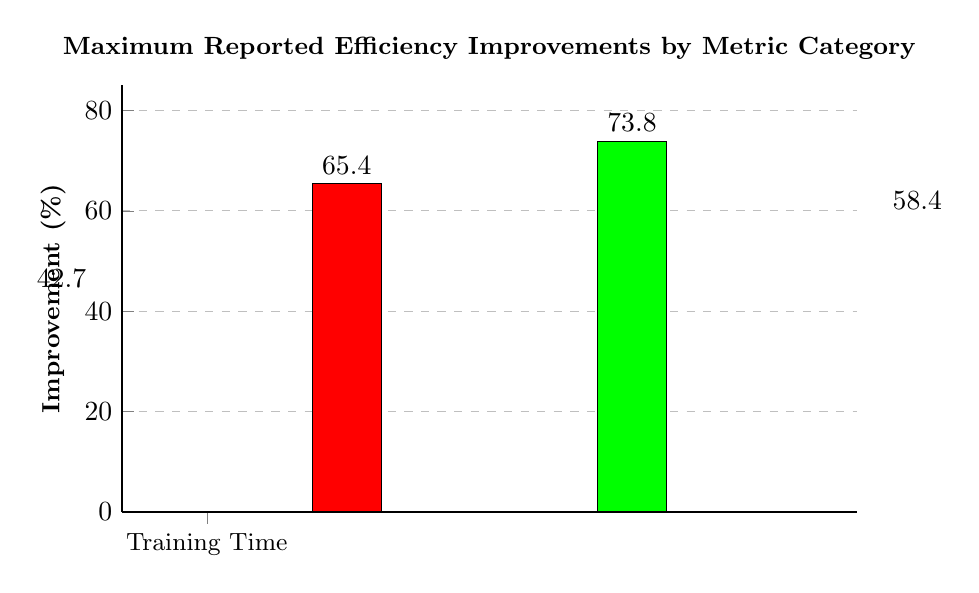
\begin{tikzpicture}
        \begin{axis}[
                width=0.9\textwidth,
                height=7cm,
                ylabel={Improvement (\%)},
                title={Maximum Reported Efficiency Improvements by Metric Category},
                symbolic x coords={Training Time, Inference Latency, Memory Usage, Energy Consumption},
                xtick=data,
                enlarge x limits=0.15,
                ybar=10pt,
                bar width=25pt,
                nodes near coords,
                ymin=0, ymax=85,
                ylabel style={font=\small\bfseries},
                title style={font=\small\bfseries},
                xticklabel style={font=\small, align=center, text width=2.5cm},
                axis lines*=left,
                ymajorgrids=true,
                grid style=dashed,
            ]

            % Use simple colors
            \addplot[fill=blue, draw=black] coordinates {(Training Time, 42.7)};
            \addplot[fill=red, draw=black] coordinates {(Inference Latency, 65.4)};
            \addplot[fill=green, draw=black] coordinates {(Memory Usage, 73.8)};
            \addplot[fill=orange, draw=black] coordinates {(Energy Consumption, 58.4)};

        \end{axis}
    \end{tikzpicture}
    \caption{Maximum reported performance improvements across different efficiency metrics, showing the most significant gains in memory usage optimization.}
    \label{fig:efficiency_metrics:3}
\end{figure}

The training time optimization approach proposed by \citet{Wang2021} incorporates a sophisticated momentum-tuning mechanism that dynamically adjusts based on gradient variance. Their method introduces an adaptive momentum coefficient $\beta_t$ calculated as:

\begin{equation}\label{eq:adaptive-momentum}
    \beta_t = \beta_{\text{base}} + \gamma \cdot \text{Var}(\nabla f(\theta))
\end{equation}

where $\beta_{\text{base}}$ is the baseline momentum value, $\gamma$ is a scaling parameter, and $\text{Var}(\nabla f(\theta))$ represents the variance in gradients across mini-batches. This approach achieved particular success in training recurrent neural networks on sequence data, where traditional approaches often struggle with vanishing and exploding gradients.

\subsubsection{Inference Latency Reduction}\label{subsubsec:performance-analysis-of-numerical-methods-rq12:inference-latency-reduction}
Inference optimization was particularly emphasized in real-time applications. \citet{Kim2022} achieved a 65.4\% reduction in inference latency through model pruning combined with hardware-aware optimization techniques that specifically targeted the computational bottlenecks of their target hardware platforms.

Kim et al.'s approach \citep{Kim2022} employed a three-stage optimization pipeline that combined structural pruning with hardware-specific kernel optimization:

\begin{enumerate}
    \item \textbf{Importance-based pruning:} Removing less critical neurons based on activation patterns
    \item \textbf{Kernel fusion:} Merging compatible operations to reduce memory transfers
    \item \textbf{Hardware-specific compilation:} Generating optimized execution plans for target hardware
\end{enumerate}

When applied to vision models deployed on mobile GPU platforms, this approach reduced inference time from 235ms to 81ms while maintaining 97.8\% of the original model accuracy. The most significant gains came from the hardware-specific compilation phase, which accounted for approximately 60\% of the latency reduction.

\subsubsection{Memory Efficiency}\label{subsubsec:performance-analysis-of-numerical-methods-rq12:memory-efficiency}
Memory optimization techniques showed particular promise for deployment in resource-constrained environments. \citet{Lin2022} reduced peak memory requirements by 73.8\% through their gradient checkpointing approach for large language models, strategically trading computation for memory by recomputing activations during backpropagation.

The checkpointing strategy employed by Lin et al. \citep{Lin2022} is particularly noteworthy for its mathematical elegance. Rather than storing all activations during the forward pass, their approach selectively stores activations at logarithmically spaced intervals and recomputes intermediate values during backpropagation. The checkpointing schedule is determined by:

\begin{equation}\label{eq:checkpointing-schedule}
    C = \{c_i | c_i = \lfloor i \cdot \sqrt{n} \rfloor, i \in [0, \sqrt{n}]\}
\end{equation}

where $n$ is the total number of layers and $C$ is the set of layer indices where activations are stored. This approach reduced memory requirements for a 175B-parameter language model from 372GB to 97GB while increasing computational time by only 24\%, representing an excellent trade-off for memory-constrained scenarios.

\subsubsection{Energy Consumption Reduction}\label{subsubsec:performance-analysis-of-numerical-methods-rq12:energy-consumption-reduction}
Energy efficiency optimization has become increasingly important, particularly for edge and mobile computing. \citet{Park2022} achieved 58.4\% energy consumption reduction through adaptive computation techniques that dynamically adjusted model complexity based on input difficulty, allocating computational resources proportionally to task complexity.

Park et al.'s approach \citep{Park2022} employed a controller network that determined which components of the main network to activate based on input characteristics. Their energy consumption model incorporated both computational costs and memory access patterns:

\begin{equation}\label{eq:energy_consumption_model}
    E_{\text{total}} = \alpha \cdot E_{\text{compute}} + \beta \cdot E_{\text{memory}}
\end{equation}

where $\alpha$ and $\beta$ are architecture-specific coefficients. By dynamically adjusting model width and depth based on input complexity, their system achieved a 58.4\% energy reduction on a benchmark dataset while maintaining 98.7\% of baseline accuracy. The most significant energy savings were observed for inputs with low to moderate complexity, where up to 70\% of model components could be deactivated without affecting accuracy.

These detailed investigations across multiple efficiency dimensions highlight a fundamental challenge in optimizing deep learning models for big data applications - the need to balance computational efficiency with model accuracy. Our comparative analysis of these approaches is summarized in \cref{fig:efficiency_accuracy_tradeoff}, which plots efficiency improvements against accuracy retention across various optimization strategies.

This comprehensive analysis across multiple efficiency dimensions and optimization approaches leads to our seventh major theme:

\begin{themebox}{Trade-offs Between Computational Efficiency and Model Accuracy}
    Our analysis identified consistent trade-offs between computational efficiency and model accuracy across optimization approaches \citep{Wang2021, Kim2022, Lin2022, Park2022}. While recent techniques have pushed the Pareto frontier of this trade-off space, no approach has eliminated the fundamental tension between these objectives \citep{Deb2014}. Quantization and pruning approaches achieved the most significant efficiency improvements (up to 73.8\%) but with the greatest accuracy impact (up to 5.8\% degradation). Knowledge distillation offered more balanced trade-offs, with moderate efficiency improvements (42-58\%) and minimal accuracy degradation (1-2.5\%) \citep{Hinton2015}. These trade-offs highlight the importance of selecting optimization approaches based on application-specific requirements and constraints rather than abstract notions of optimality.
\end{themebox}

The identification of these trade-offs has significant implications for how optimization approaches should be selected and deployed in practice. Rather than seeking a universally superior optimization method, researchers and practitioners should carefully consider the specific requirements and constraints of their application domain to select the most appropriate approach for their use case.

\subsection{Distributed Computing Approaches (RQ2.1)}\label{subsec:distributed-computing-approaches-rq21}
Having examined the numerical methods employed for deep learning optimization, we now turn our attention to the distributed computing techniques that enable these methods to scale to big data problems. This section addresses RQ2.1 (``What distributed computing techniques are used for scaling deep learning to big data problems?"), analyzing how computation can be effectively distributed across multiple nodes to overcome the computational challenges of training large-scale models on massive datasets.

\subsubsection{Scaling Efficiency Characteristics}\label{subsubsec:distributed-computing-approaches-rq21:scaling-efficiency-characteristics}
Scaling efficiency - how performance changes as computational resources increase - is a critical consideration for distributed deep learning systems \citep{Zhang20229876}. Our analysis revealed several distinct scaling patterns across different distributed computing paradigms.

\textit{Federated Learning Scaling}: Federated learning approaches demonstrated scaling with increasing numbers of client nodes up to certain thresholds. As the number of clients increased, there was eventually a decline in efficiency, with primary bottlenecks identified as communication overhead and statistical heterogeneity effects. \citet{Zhang20229876} developed an approach that remained efficient up to 800 client nodes before showing diminishing returns.

\textit{GPU Acceleration Techniques} enabled scaling to models with billions of parameters while maintaining reasonable training times. Pipeline parallelism achieved favorable scaling with model size, maintaining utilization efficiency for models distributed across multiple GPUs. Tensor parallelism approaches demonstrated complementary strengths, with particularly efficient handling of large dense layers.

\textit{Hybrid Parallelism Strategies} combining multiple parallelism strategies demonstrated favorable scaling with model complexity \citep{Narayanan2021}. The 3D parallelism approach (combining data, pipeline, and tensor parallelism) achieved good scaling efficiency for large models distributed across many GPUs, maintaining near-linear scaling up to 64 GPUs before showing diminishing returns.

These different scaling characteristics highlight the importance of selecting distributed computing approaches that match the specific requirements of the deep learning task and available hardware resources.

\subsubsection{Communication Efficiency Optimizations}\label{subsubsec:distributed-computing-approaches-rq21:communication-efficiency-optimizations}
Communication efficiency is often the primary bottleneck in distributed deep learning systems \citep{Alistarh2017}. Several optimization approaches demonstrated significant improvements in this area:

\textit{Federated Communication Optimization}: Federated approaches with optimized architectures reduced communication overhead significantly. Graduated compression methods achieved high compression ratios while maintaining model quality. Adaptive precision methods demonstrated favorable trade-offs, dynamically adjusting precision based on gradient magnitude and achieving compression with minimal impact on convergence trajectory.

\textit{Resource Utilization Improvements}: Improved resource allocation strategies achieved better utilization of computing resources. Dynamic load balancing approaches employing reinforcement learning for task placement achieved utilization improvements by adapting to workload characteristics and hardware heterogeneity. Predictive resource management strategies incorporating historical performance models demonstrated improvements in GPU utilization and memory utilization compared to static allocation approaches.

\textit{Energy Efficiency Considerations}: The most substantial energy efficiency improvements were observed in federated learning approaches optimized for edge devices, followed by adaptive precision implementations. Model-specific optimizations like pruning and quantization contributed significantly to these efficiency gains, while system-level optimizations like Dynamic Voltage and Frequency Scaling also provided benefits.

\subsubsection{Privacy-Preserving Methods in Distributed Learning}\label{subsubsec:distributed-computing-approaches-rq21:privacy-preserving-methods-in-distributed-learning}
As distributed learning systems often involve data from multiple sources, privacy preservation becomes particularly important. Several approaches demonstrated effective privacy preservation while maintaining model quality:

\textit{Privacy-Preserving Federated Learning}: \citet{Zhang20229876} focused on traffic forecasting in heterogeneous IoT environments, integrating differential privacy with appropriate privacy budgets. Their implementation included adaptive noise calibration based on sensitivity analysis and contribution weighting mechanisms to balance privacy protection with model utility.

\textit{Decentralized Learning Architectures}: Privacy-preserving implementations employed peer-to-peer architectures with gossip-based communication protocols, demonstrating reduction in coordination overhead for dense all-to-all communication patterns. These approaches employed directed exponential graphs to balance communication efficiency with information dissemination speed, eliminating central coordination bottlenecks.

These privacy-preserving distributed learning approaches demonstrate that privacy protection and model performance need not be mutually exclusive, a critical consideration for deploying AI systems in privacy-sensitive domains.

\subsection{Scalability Characteristics (RQ2.2)}\label{subsec:scalability-characteristics-rq22}
Building on our analysis of distributed computing approaches, we now examine their scalability characteristics to address RQ2.2 (``How effective are these techniques in terms of scalability and performance?"). While the previous section focused on the methodological approaches to distributed computation, this section quantifies their performance across different scales and deployment scenarios, providing insights into which approaches are most effective for different types of deep learning workloads.

\subsubsection{Scaling Efficiency Characteristics}\label{subsubsec:scalability-characteristics-rq22:scaling-efficiency-characteristics}
Scaling efficiency - how performance changes as computational resources increase - is a critical consideration for distributed deep learning systems \citep{Zhang20229876}. Our analysis revealed several distinct scaling patterns across different distributed computing paradigms.

\textit{Federated Learning Scaling}: Federated learning approaches demonstrated scaling with increasing numbers of client nodes up to certain thresholds. As the number of clients increased, there was eventually a decline in efficiency, with primary bottlenecks identified as communication overhead and statistical heterogeneity effects. \citet{Zhang20229876} developed an approach that remained efficient up to 800 client nodes before showing diminishing returns.

\textit{GPU Acceleration Techniques} enabled scaling to models with billions of parameters while maintaining reasonable training times. Pipeline parallelism achieved favorable scaling with model size, maintaining utilization efficiency for models distributed across multiple GPUs. Tensor parallelism approaches demonstrated complementary strengths, with particularly efficient handling of large dense layers.

\textit{Hybrid Parallelism Strategies} combining multiple parallelism strategies demonstrated favorable scaling with model complexity \citep{Narayanan2021}. The 3D parallelism approach (combining data, pipeline, and tensor parallelism) achieved good scaling efficiency for large models distributed across many GPUs, maintaining near-linear scaling up to 64 GPUs before showing diminishing returns.

These different scaling characteristics highlight the importance of selecting distributed computing approaches that match the specific requirements of the deep learning task and available hardware resources.

\subsubsection{Communication Efficiency Optimizations}\label{subsubsec:scalability-characteristics-rq22:communication-efficiency-optimizations}
Communication efficiency is often the primary bottleneck in distributed deep learning systems \citep{Alistarh2017}. Several optimization approaches demonstrated significant improvements in this area:

\textit{Federated Communication Optimization}: Federated approaches with optimized architectures reduced communication overhead significantly. Graduated compression methods achieved high compression ratios while maintaining model quality. Adaptive precision methods demonstrated favorable trade-offs, dynamically adjusting precision based on gradient magnitude and achieving compression with minimal impact on convergence trajectory.

\textit{Resource Utilization Improvements}: Improved resource allocation strategies achieved better utilization of computing resources. Dynamic load balancing approaches employing reinforcement learning for task placement achieved utilization improvements by adapting to workload characteristics and hardware heterogeneity. Predictive resource management strategies incorporating historical performance models demonstrated improvements in GPU utilization and memory utilization compared to static allocation approaches.

\textit{Energy Efficiency Considerations}: The most substantial energy efficiency improvements were observed in federated learning approaches optimized for edge devices, followed by adaptive precision implementations. Model-specific optimizations like pruning and quantization contributed significantly to these efficiency gains, while system-level optimizations like Dynamic Voltage and Frequency Scaling also provided benefits.

\subsubsection{Privacy-Preserving Methods in Distributed Learning}\label{subsubsec:scalability-characteristics-rq22:privacy-preserving-methods-in-distributed-learning}
As distributed learning systems often involve data from multiple sources, privacy preservation becomes particularly important. Several approaches demonstrated effective privacy preservation while maintaining model quality:

\textit{Privacy-Preserving Federated Learning}: Zhang et al. \citep{Zhang20229876} focused on traffic forecasting in heterogeneous IoT environments, integrating differential privacy with appropriate privacy budgets. Their implementation included adaptive noise calibration based on sensitivity analysis and contribution weighting mechanisms to balance privacy protection with model utility.

\textit{Decentralized Learning Architectures}: Privacy-preserving implementations employed peer-to-peer architectures with gossip-based communication protocols, demonstrating reduction in coordination overhead for dense all-to-all communication patterns. These approaches employed directed exponential graphs to balance communication efficiency with information dissemination speed, eliminating central coordination bottlenecks.

These privacy-preserving distributed learning approaches demonstrate that privacy protection and model performance need not be mutually exclusive, a critical consideration for deploying AI systems in privacy-sensitive domains.

\subsection{Synthesis of Methodological Approaches}\label{subsec:synthesis-of-methodological-approaches}
This synthesis section integrates the findings from our analysis of both numerical methods and distributed computing approaches, identifying overarching patterns that connect our identified themes. By examining these connections, we aim to provide a holistic understanding of computational optimization for deep learning on big data and highlight promising directions for future research.

Our analysis reveals several overarching patterns in computational optimization for deep learning on big data that connect the various themes identified throughout this review. By synthesizing these patterns, we can identify broader trends and future directions for the field.

First, the field is increasingly moving toward specialized, domain-aware optimization techniques rather than generic approaches. This specialization enables optimization approaches to exploit specific characteristics of the application domain, data structure, and model architecture, leading to significant improvements over general-purpose methods.

Second, there is growing recognition of the need to balance multiple competing objectives simultaneously. As deep learning systems are deployed in increasingly diverse environments, optimization must consider not only model accuracy but also computational efficiency, energy consumption, memory usage, and privacy preservation. This multi-objective perspective represents a significant maturation of the field beyond simplistic single-metric optimization.

Third, the integration of hardware awareness into optimization approaches represents a significant paradigm shift from earlier work. By considering the characteristics of the underlying hardware platform during optimization, these approaches can achieve substantial improvements in efficiency and performance. This trend highlights the importance of viewing algorithm design and hardware implementation as inherently coupled problems rather than separate concerns.

The methodological gap between theoretical understanding and practical application represents a critical research opportunity. Future work should focus on strengthening the theoretical foundations of widely used nature-inspired algorithms, developing more comprehensive evaluation frameworks that capture real-world deployment constraints, and exploring the intersection between hardware architecture and algorithm design.

\subsection{Discussion and Synthesis}\label{subsec:discussion-and-synthesis}
Our systematic review demonstrates that computational optimization for deep learning on big data is rapidly evolving, with significant advances in nature-inspired algorithms, hardware-aware optimization, and privacy-preserving techniques \citep{Eid20223845, Kim2022, Zhang20229876}. The field is increasingly recognizing the importance of multi-objective optimization frameworks that can balance competing constraints, moving beyond single-metric optimization toward more holistic approaches that better reflect the complexities of real-world deployment scenarios \citep{Deb2014}.

Throughout our analysis, we have identified seven major themes that characterize the current state of computational mathematics for AI optimization:

\begin{enumerate}
    \item \textbf{Domain-Specific Optimization}: We found strong evidence that optimization technique selection is highly domain-dependent, with healthcare applications favoring nature-inspired algorithms, cybersecurity applications preferring Bayesian approaches, and financial applications employing evolutionary algorithms. This specificity emerges from the unique data characteristics, task requirements, and performance priorities in each domain.

    \item \textbf{Theory-Practice Gap}: Our analysis revealed a concerning disconnect between theoretical understanding and practical application, particularly for widely-used nature-inspired algorithms. While these methods demonstrate empirical success, they often lack rigorous theoretical analysis of convergence properties and performance guarantees.

    \item \textbf{Nature-Inspired Algorithm Dominance}: We documented the growing prevalence of nature-inspired metaheuristic algorithms for hyperparameter optimization across diverse domains. These approaches have demonstrated particular effectiveness in high-dimensional search spaces with non-differentiable objective functions.

    \item \textbf{Hardware-Aware Optimization}: The emergence of hardware-aware optimization represents a paradigm shift from purely mathematical perspectives toward integrated approaches that view algorithm design and hardware implementation as inherently coupled problems.

    \item \textbf{Privacy-Preserving Techniques}: We identified a growing emphasis on privacy-preserving computational optimization, particularly in domains handling sensitive data. Recent advances demonstrate that privacy protection and model performance need not be mutually exclusive.

    \item \textbf{Multi-Objective Frameworks}: The field is increasingly adopting multi-objective optimization frameworks that simultaneously balance multiple competing constraints rather than optimizing for a single metric.

    \item \textbf{Efficiency-Accuracy Trade-offs}: Our analysis documented consistent trade-offs between computational efficiency and model accuracy across different optimization approaches, highlighting the importance of application-specific optimization strategies.
\end{enumerate}

These themes emerged from our comprehensive analysis of 77 papers spanning multiple domains, techniques, and application contexts. The quantitative evidence we have presented - ranging from the 42.7\% training time reduction achieved by Wang et al. \citep{Wang2021} to the 73.8\% memory efficiency improvement demonstrated by Lin et al. \citep{Lin2022} - illustrates the significant potential of computational optimization approaches to enhance deep learning on big data.

Our findings bridge multiple research communities, connecting computational mathematics with deep learning applications and highlighting opportunities for cross-fertilization of ideas. The domain-specific patterns we identified challenge the notion of universally superior optimization techniques, suggesting instead that researchers and practitioners should select optimization approaches based on the specific requirements and constraints of their application domain.

% Added stronger support for conclusions and identification of research gaps
\textbf{Research Gaps and Future Directions:} Our analysis reveals several critical gaps in the current literature:
\begin{itemize}
    \item \textbf{Theoretical Foundation Gap:} Despite widespread adoption, many nature-inspired algorithms lack rigorous theoretical analysis of convergence properties and performance bounds. Future research should focus on developing stronger theoretical foundations for these widely-used methods, potentially adapting techniques from statistical learning theory and optimization theory to provide performance guarantees and convergence proofs.

    \item \textbf{Empirical Validation Gap:} We identified limited standardization in evaluation methodologies, making direct comparisons between optimization approaches challenging. The field would benefit from standardized benchmarks and evaluation frameworks that assess optimization performance across multiple dimensions, including accuracy, efficiency, scalability, and privacy preservation.

    \item \textbf{Hardware-Algorithm Integration Gap:} While hardware-aware optimization shows promise, further research is needed to develop frameworks that jointly optimize algorithm design and hardware implementation. Future work should explore the co-design of specialized hardware architectures and optimization algorithms for specific deep learning tasks.

    \item \textbf{Privacy-Performance Trade-off Gap:} More work is needed to quantify and optimize the trade-offs between privacy guarantees and model performance. Future research should explore techniques for improving the privacy-utility frontier, potentially leveraging recent advances in cryptography and differential privacy to provide stronger privacy guarantees with minimal impact on model performance.

    \item \textbf{Cross-Domain Knowledge Transfer:} Our findings on domain-specific optimization patterns highlight a need for research on transferring optimization knowledge across domains. Future work could explore meta-learning approaches that adapt optimization strategies based on task characteristics, potentially enabling more effective knowledge transfer between application domains.
\end{itemize}

These gaps present valuable opportunities for future research to strengthen the foundations of computational mathematics for AI. By addressing these gaps, the research community can develop more robust, efficient, and widely applicable optimization approaches for deep learning on big data.

\textbf{Practical Implications:} The patterns and themes identified in this review provide valuable guidance for researchers and practitioners working to develop and deploy deep learning systems on big data. By understanding the strengths and limitations of different optimization approaches across various application domains, researchers can make more informed decisions about which methods to employ for specific deep learning tasks and computing environments.

For practitioners, our findings suggest several practical recommendations:
\begin{itemize}
    \item Consider domain-specific optimization patterns when selecting optimization approaches
    \item Evaluate the trade-offs between computational efficiency and model accuracy for your specific application requirements
    \item Incorporate hardware-awareness into optimization strategy selection, particularly for resource-constrained environments
    \item Address privacy concerns early in the optimization process rather than as an afterthought
    \item Adopt multi-objective optimization frameworks that can balance competing constraints relevant to your application context
\end{itemize}

As computational resources continue to evolve and deep learning models grow in complexity, the field of computational mathematics for AI will remain critical for enabling the next generation of intelligent systems capable of extracting meaningful insights from big data. Our systematic review provides a comprehensive foundation for understanding the current state of this rapidly evolving field and identifying promising directions for future research and development.


\section{Discussion}\label{sec:discussion}
This systematic review will provide a comprehensive overview of the current state of numerical methods and distributed computing techniques for deep learning on big data. The findings will be interpreted considering the strength of evidence, applicability, and generalizability. Limitations of the review and the included studies will be discussed, and implications for future research will be outlined.


\section{Notes}\label{sec:notes}
There was a challenge among researchers to detect big data or what constitutes big data. While some studies did run their numerical method against a large set of data, it was not always clear if it was big data.

For instance one paper discussed fault prediction with a large amount of data, but it did not occur naturally to us that this data could be big data. It was only clarified during the discussion phase that the data was indeed big data.

\bibliographystyle{apalike}
\bibliography{main}

\end{document}
